% =============================================================================
% manuscript.tex — Environmental Modelling & Software (Elsevier), elsarticle class
%
% GENERATED FILE. Do not edit by hand: it is produced from the Markdown sources
% by paper/tex/build_tex.mjs. Edit the Markdown and re-run the script, or the
% next build will silently discard your changes.
%
% Build:  pdflatex manuscript && bibtex manuscript && pdflatex manuscript x2
% Needs:  elsarticle.cls and elsarticle-harv.bst (TeX Live / MiKTeX / Overleaf)
%
% COMPILED. First compiled 2026-08-14 with MiKTeX 25.12 (pdfTeX), clean: no
% errors, no undefined references, no undefined citations. The first compile was
% a debugging pass and found four real defects, all fixed in this generator: a
% true minus inside a code span (the Unicode table was applied to prose but not
% to code spans), non-ASCII inside a verbatim block, figure paths resolved from
% the wrong directory, and l-columns that cannot wrap, which ran the widest
% table 763pt past the margin. See build_report.md.
% =============================================================================
%% authoryear is required by elsarticle-harv. Without it citep printed a
%% bracketed number while the reference list stayed alphabetical author-year,
%% so the in-text numbers ran 29, 42, 14 with nothing to match them against.
\documentclass[preprint,review,authoryear,12pt]{elsarticle}

\usepackage[utf8]{inputenc}
\usepackage[T1]{fontenc}
\usepackage{lmodern}
\usepackage{textcomp}
\usepackage{tabularx}
\graphicspath{{../}{../figures/}{./}{./figures/}}
\usepackage{graphicx}
\usepackage{amsmath}
\usepackage{booktabs}
\usepackage{longtable}
\usepackage{array}
\usepackage{url}
%% The review option double-spaces everything, captions included. A 267-word
%% caption then stands 160 mm tall, which together with the figure exceeds the
%% 193 mm text block, and the folio prints through the caption text. LaTeX
%% reports no overfull box for it, because the float is allowed to be tall.
%% Captions are set at normal leading, as journals set them.
%% Long 	exttt file names are broken at llowbreak points, but TeX was still
%% choosing lines that ran up to 10 mm past the right margin rather than
%% stretching the spaces, and was not reporting them as overfull. emergencystretch
%% gives it a third pass in which a loose line is preferred to a protruding one.
\emergencystretch=3em
\usepackage{setspace}
\usepackage{etoolbox}
\AtBeginEnvironment{figure}{\singlespacing}
\AtBeginEnvironment{table}{\singlespacing}
\usepackage{lineno}
\modulolinenumbers[5]

\journal{Environmental Modelling and Software}

\begin{document}

\begin{frontmatter}

%% Title. POSITIONING.md lists three candidates and directs that under Branch A
%% (Evia enlarged and re-run cleanly, which is what happened) the third is used.
%% Referee round 2, 2026-08-14: that third candidate began "Marginal diagnostics
%% miss conditional failures", which asserts more than Section 5.4 concedes. On
%% ten effective pairs the null diagnostics are "not shown to order transfer",
%% not "shown not to". The title now says what Section 4.4 found and what
%% Section 5.4 defends. Candidate 1 was not used because "do not transfer
%% between them" is contradicted by the paper's own matrix, and candidate 2 was
%% not used because "transferability cost" asserts a debit measured only by the
%% feature-removal ablation. Change here if that decision is revisited.
%% Retitled 2026-08-14 in the split, to carry the three findings the paper was
%% cut to. "Sign reversal" names the mechanism, which the old title left out;
%% "do not order" is kept verbatim because it is the only claim Section 5.4
%% defends, the diagnostics having been shown not to order transfer here rather
%% than shown incapable of ordering it anywhere.
\title{Evaluation geometry and the limits of cross-region transfer in pre-fire thermal wildfire prediction}

%% Author block. Affiliation and corresponding address supplied by the authors
%% 2026-08-14. Order changed 2026-08-15 on the authors' instruction: Emrehan
%% Metin first, Yunus Emre Cogurcu second. Corresponding authorship was NOT
%% moved with it and stays with Cogurcu, who supervises the work and whose
%% address is the one on file; say so if that is not intended.
%% Still optional and not supplied: department or faculty within the
%% university, and ORCIDs.
\author[inst1]{Emrehan Metin}
\author[inst1]{Yunus Emre Cogurcu\corref{cor1}}
\ead{ycogurcu@cu.edu.tr}
\cortext[cor1]{Corresponding author.}
\affiliation[inst1]{organization={\c{C}ukurova University},
                    city={Adana},
                    country={T\"urkiye}}

\begin{abstract}
We test whether six pre-fire thermal predictors, added to a terrain, fuel and greenness baseline, transfer between five Mediterranean regions under MCD64A1 labels and spatially blocked validation. The first result is \textbf{evaluation geometry}: with the model held fixed, scoring on the burn scar and its 2 km collar rather than region-wide costs \textbf{0.133 ROC-AUC [+0.059, +0.207]}. Equalising the study areas to a 10 km collar lifts mean transfer from 0.527 to 0.589. Local skill does not travel: the thermal block adds +0.045 to +0.148 within regions at 5 km blocking but +0.007 [$-$0.021, +0.037] across twenty directions, and the static baseline transfers no better, at 0.519 against 0.527. At the point estimates, similarity is neither sufficient nor necessary: the most niche-similar pair fails both ways (0.438, 0.345), the least similar transfers above chance (0.594, 0.548). Transfer skill must be measured on the target region before a model is relied on.
\end{abstract}

\begin{highlights}
  \item Scoring the same model at the fire, not region-wide, costs 0.133 AUC
  \item The cause is the negative pool, not prevalence: +0.149 against -0.002
  \item Equalising the evaluation frame lifts mean transfer from 0.527 to 0.589
  \item Across 20 transfer directions the thermal gain is +0.007 [-0.021, +0.037]
  \item Highest niche-overlap pair fails both ways; lowest-overlap pair transfers both ways
\end{highlights}

\begin{keyword}
wildfire \sep model transferability \sep model evaluation \sep land surface temperature \sep domain adaptation \sep concept shift
\end{keyword}

\end{frontmatter}

\linenumbers

\section{Introduction}\label{sec:1}

Wildfire is a defining disturbance of Mediterranean-basin landscapes, and a changing climate is reshaping where and how it burns \citep{Pausas2021}. The dominant pattern in fire susceptibility mapping \citep{Vibhandik2026,Jodhani2026} is settled. Geospatial predictors are assembled over a study region, paired with a historical burned-area record and fitted with a supervised classifier, most often a random forest \citep{Breiman2001}. The surface is then published with a cross-validated AUC of 0.85 to 0.95. \textbf{That pattern does not report portability}, and this paper measures it.

\subsection{Portability goes unmeasured}\label{sec:1.1}

A susceptibility model's reported skill is almost always a \emph{within-region} estimate: held-out folds come from the same study area and season, often the same fire, and random folds over cells let spatial autocorrelation inflate it further. The problem is documented across ecological modelling \citep{Roberts2017,Ploton2020} and addressed by spatially blocked cross-validation \citep{Valavi2019,Meyer2018}, but blocking does not make the estimate honest about a fire the model has not seen.

Because only that side of the ledger is reported, portability is never entered. A predictor block is adopted on the increment it delivers inside its training footprint, and whether that survives a change of region is not asked. Yet any regional product built from locally trained models implicitly promises generalisation beyond it. Meteorological fire-danger indices are known not to port cleanly in a Peruvian case study \citep{Podschwit2022}. The two studies that test transfer systematically \citep{Dimarco2026,Liu2025} both report that it largely succeeds between similar regions. Both transfer models whose dominant predictors are \emph{spatially stationary}. Whether a dynamic, season-specific class behaves the same way is this paper's question.

\subsection{Pre-fire thermal dryness is the natural test case}\label{sec:1.2}

Pre-fire thermal dryness is the dynamic class most plausibly \emph{expected} to transfer. Standard predictors are static or near-static over the timescale at which fire danger varies, so they explain poorly why one summer burned and the preceding one did not. What changes is the state of the surface, to which satellite thermal observation gives partial access (Section~\ref{sec:2.2}). The physics linking moisture stress to combustion is universal, so portability should be most expected here, which makes the class diagnostic: a loss cannot be dismissed as a peculiarity of a locally defined covariate. The expectation is sharpest for the internally normalised channels, which should be least exposed to absolute-temperature offsets between regions; \textbf{they transfer no better than the absolute ones} (Appendix A(f)). The expectation motivates the design and is not a finding of it --- Section~\ref{sec:4.4} reports the associations running the other way.

\subsection{Contributions}\label{sec:1.3}

Three findings carry this paper, stated here as claims and established in Section~\ref{sec:4}, which carries every interval.

\textbf{Contribution 1. Where a model is scored decides what it appears to know, and the effect is large enough to dissolve findings of our own.} That evaluation extent inflates AUC is established in species distribution modelling (Section~\ref{sec:2.4}). What is new is a magnitude under a controlled design. Holding model, predictors and fitting fixed and changing only which cells are scored costs \textbf{0.133 ROC-AUC}, the size of the increments this design measures for a predictor block. The cause is measured as the composition of the negative pool rather than class balance (Section~\ref{sec:4.3}), and the cost holds with the region as the resampling unit. Applied between regions, the same test shows four of our own quantities to be properties of the frames, including the one arm that held place fixed (Section~\ref{sec:4.4}). One reversal survives it, Manavgat's elevation. The practical consequence is a reporting standard (Section~\ref{sec:5.6}).

\textbf{Contribution 2. Local skill does not travel, and correcting the frame does not rescue it.} The thermal block is worth a substantial within-region increment in all five regions, every bootstrap interval above zero, and it stays positive when the frame is equalised. At the scar level much of it is a property of interleaved holdout; clustered by region, that part is not established (Section~\ref{sec:4.3}). Across twenty transfer directions the paired contribution spans zero on both frames under the primary resampling unit. Once equalised it lies much closer to the boundary, and under one admissible unit, clustering by target region, it excludes zero (Section~\ref{sec:4.4}). Its sign belongs to the pair rather than the block. Two controls bound this. The static baseline transfers no better on either frame, so the failure is not the thermal block's peculiarity. On matched frames and blocking, equalised transfer still falls \textbf{0.197} short of the within-region reference. The within-region half is not novel \citep{AlkanAkinci2023,Iban2022}; the paired contrast against portability is.

\textbf{Contribution 3. No similarity diagnostic we tested is shown to order transfer, conditional ones included.} Twenty measures were fixed in advance. They range from marginal covariate distance through niche overlap and regime structure to the conditional agreement of predictor--burning relationships. Under the corrected label nineteen have correlation intervals spanning zero. The twentieth is defined in only six directions, with a degenerate interval, and is not interpreted (Section~\ref{sec:4.6}, Appendix D). The conditional measure that had ordered transfer under the frozen label ($\rho$ = +0.84) no longer does (+0.52 [$-$0.27, +0.87]). With ten effective region pairs this is a failure to show ordering, not proof that none exists. The practical consequence is that no pre-deployment shortcut replaces measuring transfer on the target.

Two consequences follow, as supporting results. Label-free alignment by standardisation and covariance alignment \citep{Sun2016} does not repair transfer, in what we believe is its first application to fire susceptibility. And because the residual is conditional, the resource that closes it is target labels, priced in Appendix A(u).

The leakage-audited, spatially blocked protocol is released with code, configuration and frozen outputs, so most of this can be re-run rather than taken on trust. The release is complete, as the declarations record. That matters given evidence that wildfire transfer conclusions are sensitive to evaluation design \citep{Xu2026}. A companion paper treats the observational layer beneath this one.



\section{Related work}\label{sec:2}

\subsection{Fire susceptibility mapping, and what it reports}\label{sec:2.1}

The dominant pattern is described in Section~\ref{sec:1}; the figure it publishes, a cross-validated AUC of 0.85 to 0.95, is a within-region estimate. Comparable within-region results already exist for the landscapes studied here \citep{AlkanAkinci2023,Iban2022}.

\subsection{Pre-fire thermal dryness}\label{sec:2.2}

Satellite thermal observation gives repeated access to surface state through fuel moisture content \citep{Yebra2013}. \citet{Chuvieco2004} established the pairing of land surface temperature with a vegetation index as a live-fuel-moisture estimator for fire-danger rating. The Temperature-Vegetation Dryness Index \citep{Sandholt2002} formalises that feature space into an internally normalised measure, which is why it is often expected to travel better than raw temperature. That pre-fire thermal state carries information about subsequent fire is established \citep{Maffei2018,MaffeiMenenti2019,Maffei2021}. \citet{Gelabert2025} found dead fine fuel moisture and its anomalies the most influential predictor of human-caused ignition likelihood across Europe, testing generalisation by pooled fitting with per-site evaluation. What has not been tested is whether such a classifier survives strict, label-free application to an unseen region.

\subsection{Spatial validation and transferability}\label{sec:2.3}

The canonical taxonomy separates covariate shift from concept shift \citep{MorenoTorres2012}. Under covariate shift the predictor distribution moves but the predictor-response relationship holds; under concept shift the relationship itself changes. Covariate shift is in principle correctable without target labels, by per-region standardisation or covariance alignment such as CORAL \citep{Sun2016}, and domain adaptation has an established remote-sensing literature \citep{Tuia2016,Persello2012}. Concept shift is not: no realignment of inputs can repair a reversal in the sign of an association, because detecting one requires the labels being withheld. Shift decomposition in applied remote sensing is not itself new \citep{Huang2026}, but we are aware of no prior application of covariance alignment to fire susceptibility, fire occurrence or burned-area prediction.

\subsection{Cross-region generalisation of fire models}\label{sec:2.4}

Few studies test fire-model transfer directly. \citet{Podschwit2022} report, in a Peruvian case study, that meteorologically derived danger indices do not port cleanly between fire environments. WildfireGenome \citep{Liu2025} runs a leave-one-county-out matrix across seven US counties, and reports strong within-county performance with highly variable off-diagonal transfer, similar pairs transferring well and dissimilar pairs collapsing. Its label is a principal-component composite of hazard \emph{indicators} rather than observed burned area, and it applies no adaptation. \citet{Xu2026} argue that wildfire transfer conclusions depend strongly on evaluation design. We address that caution in two ways: the protocol was fixed in a project log before the diagnostics were computed, and every sensitivity axis is reported. That log is not a formal pre-registration, and Appendix D states what was fixed and when. \citet{Kondylatos2023} provide Mesogeos, a 1 km Mediterranean datacube.

\textbf{Evaluation extent and AUC.} Species distribution modelling settled long ago that the area a model is evaluated over is not a neutral choice. \citet{Lobo2008} make it the fifth and, by their own ranking, most important reason to distrust AUC comparatively. The extent of the modelled area governs how many easy absences enter the calculation, and therefore the score. \citet{VanDerWal2009} show the same lever on the calibration side, and \citet{Barve2011} give the argument its general form as the accessible area. That literature is qualitative about magnitude, because magnitude is problem-specific, so our Contribution 1 is a measurement inside that framework rather than a new phenomenon. The wildfire literature has largely not imported the lesson: region-wide figures are reported as though they described performance at the fire. We know of no wildfire study that holds the model fixed and varies only the evaluation cells. That is why Section~\ref{sec:5.6} treats the 0.133 as a reporting problem rather than a caveat.

\textbf{The nearest neighbour, and the contrast this paper draws.} \citet{Dimarco2026} is the closest Mediterranean analogue. They harmonise 500 m predictors across four countries and fit tree ensembles under spatial cross-validation. Transfer is tested both leave-one-country-out and as a full 4 $\times$ 4 matrix. Every transfer exceeds AUC 0.80, bioclimatically similar countries score higher, and no domain adaptation is used.\footnote{Their Results text refers to ``LST anomalies'', inconsistent with their own Methods, where no land surface temperature or TVDI variable appears and the only temperature predictor is a static ERA5-Land seasonal climatology \citep{MunozSabater2021}. We follow their Methods and note the discrepancy so the comparison is transparent.} Much of the design is shared: Mediterranean regions, 500 m cells, MCD64A1-derived targets, tree ensembles, spatially aware validation and an explicit transfer matrix; two things differ. \textbf{The predictor class}: their model rests on attributes of a place, all spatially stationary, ours on the state of a surface in one season. \textbf{The response variable}: theirs is human-driven ignition, ours burned area, which have different dominant controls. Read together, the two results suggest the relationship between domain similarity and transfer success may be predictor-class dependent. \citet{Vesk2021} and \citet{Rousseau2022} align with that reading from species distribution modelling, while Dimarco et al. and WildfireGenome run against it. We present that as a live disagreement; Section~\ref{sec:5.5} states why our data do not settle it.




\section{Data and methods}\label{sec:3}

\subsection{Study regions and temporal windows}\label{sec:3.1}

Five Mediterranean wildfire regions are analysed (Fig.~\ref{fig:study-map}): Manavgat 2021 and Muğla 2021 in Türkiye, Bejís 2022 in Spain, North Evia 2021 in Greece and Montiferru 2021 in Sardinia. Each is a place-based rectangle in EPSG:4326, defined from place coverage rather than from a fire perimeter and deliberately not clipped to it, so that unburned cells around each fire form the negative class. \textbf{The record does not show every box fixed before any outcome was seen}, so what it does show is stated region by region. In the pipeline's version history each box has a single committed value, never changed afterwards. Montiferru's is derived deterministically from the union of four municipal boundaries. Manavgat's was drawn to exclude the coastal cropland belt; its final coordinates are in a dated AOI preview record of 7 July 2026, the day before its first gate result, and never changed. Bejís's is still labelled the initial candidate in the registry but was committed after its first gate and model results. Muğla's coordinates appear in a dated preflight record about four minutes before its first gate result and were committed to the registry only afterwards. No box needed adjusting to pass the gate, whose admitted margins are wide (Section~\ref{sec:4.1}). \textbf{One choice was label-informed and is stated as such}: the North Evia box was extended after the legacy box proved atypically high in burned prevalence, the extended geometry then defined from place anchors and the legacy variant kept as a sensitivity arm. Section~\ref{sec:4.4} shows this framing decision is consequential and Appendix C.5(ix) treats it as the design lesson of the paper. A sixth region, Kozan 2023, is carried as a negative control and excluded by the gate of Section~\ref{sec:3.3}.

\begin{figure}[htbp]
  \centering
  \makebox[\linewidth][c]{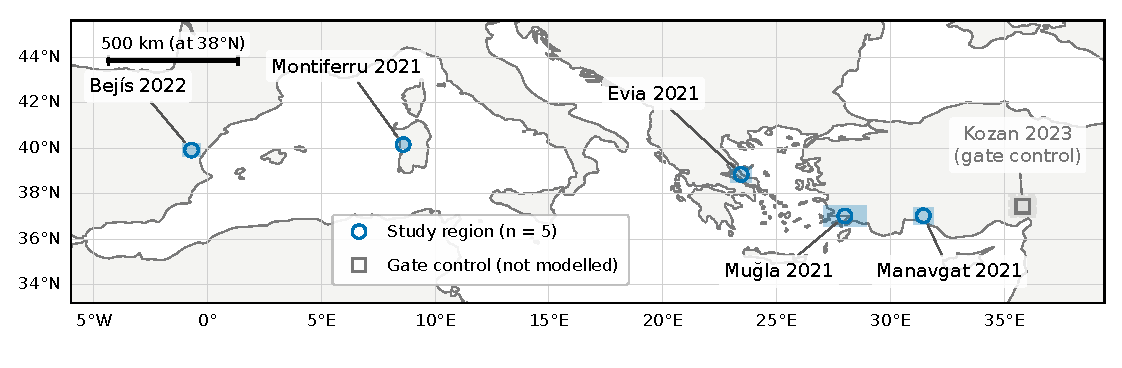
\includegraphics[width=140mm]{figures/fig1_study_map.pdf}}
  \caption{\textbf{Study regions and the gate negative control.} Locations of
  the five wildfire regions analysed in this study (blue, circular markers):
  Manavgat 2021 and Mu\u{g}la 2021 (T\"urkiye), Bej\'is 2022 (Spain), North
  Evia 2021 (Greece, extended AOI) and Montiferru 2021 (Sardinia, Italy).
  Rectangles are the true analysis areas of interest; the ring marks each
  centroid, because at basin scale the rectangles alone are hard to locate.
  Kozan 2023 (grey, dashed outline, square marker) is \emph{not} a study
  region: it is the negative control used to calibrate the burned-landcover
  admissibility gate, and it enters no model, transfer or diagnostic anywhere
  in this paper. Its rectangle is the true extent of its processed AOI and is
  larger than the study AOIs for that reason alone; the difference in size
  carries no methodological meaning and is not a design choice. Coastlines are
  Natural Earth 1:50\,m; country borders are omitted deliberately. The scale
  bar is exact only at 38\textdegree N. Region bounding boxes match Table~C1 to
  $5\times10^{-3}$ degrees.}
  \label{fig:study-map}
\end{figure}

Each region has two non-overlapping windows. The \textbf{predictor window} closes the day before the \textbf{label window} opens, so no predictor observation can post-date the first labelled burning. Lengths vary with the event: 57 to 61 days for predictors, 35 to 59 for labels, counted inclusively. A four-year baseline of window-symmetric composites precedes each predictor window and supplies the climatological reference for the anomaly channels. Region identifiers, bounding boxes, window dates and baseline years are registered in \texttt{core/\allowbreak{}regions.\allowbreak{}py} and reproduced in Appendix C, Table C1. The processing chain and the evaluation programme it feeds are drawn in Fig.~\ref{fig:pipeline}.

\begin{figure}[htbp]
  \centering
  \makebox[\linewidth][c]{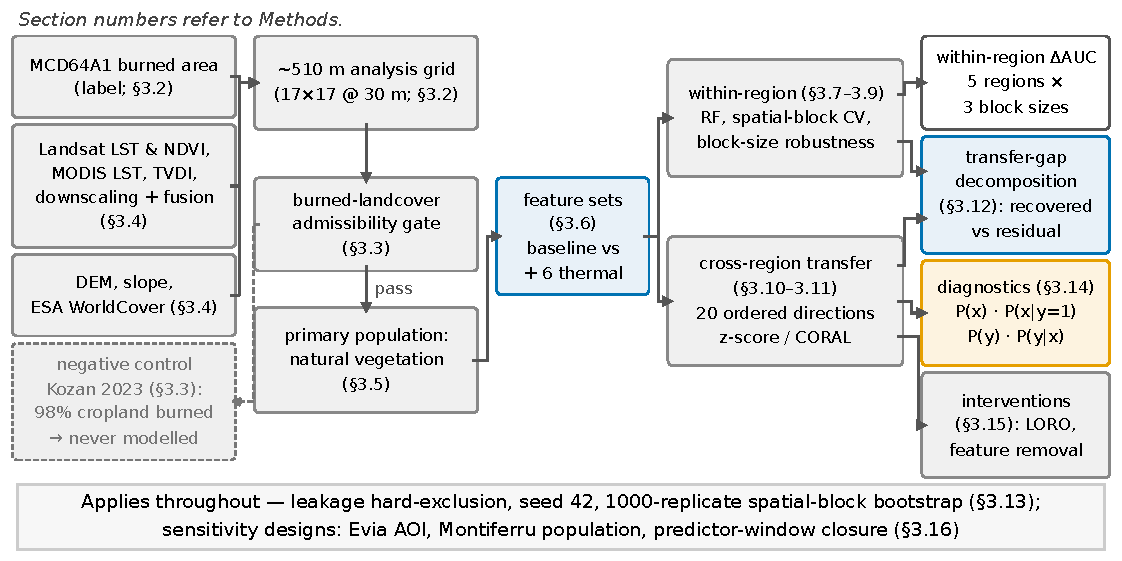
\includegraphics[width=140mm]{figures/fig2_schematic.pdf}}
  \caption{\textbf{Processing pipeline and evaluation programme.} Flow from
  source products (left) to the transfer and diagnostic programme (right);
  every box carries the Methods subsection that specifies it. The five source
  products (MCD64A1 burned area, Landsat Collection 2 Level-2, MOD11A1,
  Copernicus DEM GLO-30 and ESA WorldCover) merge onto the reconstructed
  $\sim$510\,m analysis grid
  ($17\times17$ pixels of the 30\,m reference grid). The burned-landcover
  admissibility gate has two outcomes: regions that \emph{pass} proceed to the
  natural-vegetation primary population, while the rejecting branch (grey,
  dashed) terminates in the Kozan 2023 negative control, whose burned area is
  98\% cropland and which is never modelled. The dashed connector deliberately
  carries no arrowhead onward, so the control cannot be read as entering the
  pipeline. Feature sets feed two evaluations in parallel: within-region
  (random forest under spatial-block cross-validation) and cross-region
  transfer (source-only, 20 ordered directions, with label-blind z-score and
  CORAL adaptation). Their levels are combined in the transfer-gap
  decomposition (\S3.12). The footer states what applies throughout: leakage
  hard-exclusion, seed 42, 1000-replicate spatial-block bootstrap (\S3.13), and
  the sensitivity designs (\S3.16). Section references are verified against the
  Methods heading list when the figure is built.}
  \label{fig:pipeline}
\end{figure}

\subsection{Burned-area label and the $\sim$500 m analysis grid}\label{sec:3.2}

Labels come from MODIS MCD64A1 Collection 6.1 \citep{Giglio2018} retrieved through Google Earth Engine \citep{Gorelick2017}, whose omission and commission characteristics \citep{Boschetti2019} bound every model here. The analysis grid is \textbf{reconstructed rather than native}: the pipeline's 30 m EPSG:4326 reference grid is partitioned into 17 x 17 blocks, giving a nominal 510 m cell that approximates rather than reproduces the MODIS cell and is square in degrees but not on the ground. A cell's burn date is the mode of its positive sub-pixel day-of-year values, tested against the label window; the label never affects eligibility for modelling. Two safeguards are recorded rather than assumed: cells burning before the label window opens are removed, which ran for three of five regions and excluded 49 cells in Muğla, 16 in North Evia and 61 in Montiferru, with none arising in Manavgat or Bejís, and burning in earlier years is screened for none. Appendix C.1 gives the full specification, including what follows from the grid's shape.

\textbf{The Manavgat 2021 label is a corrected one.} The label first used for Manavgat was exported on 8 July 2026. That was before the month-alignment fix to the MCD64A1 query (commit 183be42, 11 July), and the export was never renewed. It therefore missed the fire's first four days, 28 to 31 July. The defect was a stale export, not a code error. The corrected label only adds burned cells. No cell burned under the original label becomes unburned, and no predictor or validity flag changes. In the primary population the burned count rises from 784 to 2,935. The Manavgat outputs were re-frozen with the upstream pipeline at commit 6381f4c, through the Earth Engine project \texttt{thermaltwin}, in Python 3.12.10 with scikit-learn 1.9.0 (pins in \texttt{ENVIRONMENT.\allowbreak{}md}). That pipeline version writes one extra column, a flag for burning in earlier years, and it excludes no Manavgat cell. A control arm re-froze the original label with the same code and environment and reproduced the published outputs to within 10$^{-5}$. The exceptions are listed in the manifest: file paths, the column list, and one legacy pair that differs at the level of random-forest thread nondeterminism. Differences between the two arms are therefore attributable to the label alone. The reproduction check of Section~\ref{sec:3.13} covers the re-frozen outputs. The manifest, hashes and runner scripts are released under \texttt{paper/\allowbreak{}data/\allowbreak{}manavgat\_\allowbreak{}2021/\allowbreak{}refreeze/\allowbreak{}}.

\subsection{Burned-landcover admissibility gate}\label{sec:3.3}

Before any modelling each region passes a gate asking what fraction of its burned cells is dominated by natural vegetation, using ESA WorldCover classes \citep{Zanaga2022} on the same cells. A region is admitted at 0.50 with at least 30 burned cells, and rejected as a cropland-dominated control at 0.50 cropland. Verdicts and the purpose of the gate are in Section~\ref{sec:4.1}, the full rule in Appendix C.1.

\subsection{Predictor variables}\label{sec:3.4}

Two feature sets are used. The \textbf{baseline} is terrain, fuel and greenness: elevation, slope, dominant land cover and a predictor-window median vegetation-index composite, all static or near-static over the timescale at which fire danger varies. The \textbf{thermal} set adds six pre-fire channels: current land surface temperature, its anomaly against a four-year window-symmetric baseline at the same cell, the Temperature-Vegetation Dryness Index and its difference against that baseline, and two coordinate-informed products, a downscaled and a fused surface temperature. The two differenced channels are the ones constructed to isolate the dynamic anomaly. TVDI's wet and dry edges are percentiles of the values a given area and window happen to contain, so \textbf{it is not portable as a physical quantity independently of any concept shift} (Appendices C.4, C.5).

\textbf{Quality screening of the coarse thermal input, and a correction.} The MODIS surface temperature behind the downscaled and fused channels entered Manavgat's frozen export unscreened. Appendix A(e) compares that arm with a screened one on the corrected label. The current pipeline's step7 refuses the unscreened raster, because it carries no nodata tag and 8.1 \% exact zeros. The unscreened arm therefore runs the step7 of export time and the screened arm the current one, so the two differ in code version as well as in screening. The earlier version of this comparison, run on 14 August 2026, described both arms as rebuilt with the same code. That was almost certainly inaccurate: its unscreened arm would have met the same refusal, and its signed AUCs equal the frozen ones. Its Muğla arm was not re-examined. The result does not change. Elevation stays at 0.232, no other signed AUC moves by more than 0.005 (downscaled LST, $-$0.0044), and the within-region increment moves from +0.067 to +0.068 (Appendix C.5(xii)).

\subsection{Cell aggregation, validity and analysis populations}\label{sec:3.5}

Cell-level values are means over the $\sim$510 m cell from valid 30 m pixels only, with the valid fraction recorded. A cell is \texttt{valid\_\allowbreak{}for\_\allowbreak{}modeling} when it is analysis-eligible, meaning not excluded for pre-label burning, and its predictors are valid: joint finite NDVI, elevation and slope support over at least 30 \% of the cell, finite means for those three channels, and at least one valid land-cover pixel. \textbf{Thermal completeness is not part of the definition}: depending on the region, 6 \% to 58 \% of valid cells carry at least one missing thermal channel, and missing values are imputed inside the fitting pipeline (Section~\ref{sec:3.6}) rather than by excluding the cell. The \textbf{primary} population is natural vegetation, cells whose combined tree, shrub and grass fraction reaches 0.50, which excludes cropland from every burnable mask. The \textbf{secondary} population is all valid cells; the frozen export carries it for the within-region arm in two regions, reported as a sensitivity in Appendix A(v), and the transfer matrix is defined on the primary population only.

\subsection{Classifier}\label{sec:3.6}

The two feature sets of Section~\ref{sec:3.4} are nested, the thermal set being the baseline plus the six thermal channels. Land cover is one-hot encoded. Missing numeric values are median-imputed and the categorical channel most-frequent-imputed, with the imputers fitted inside each training fold, and on the source alone in transfer, so no held-out statistic enters a fit in the raw arms. Features are not otherwise standardised. Standardisation appears only in the adapted arms of Section~\ref{sec:3.9}, where target feature statistics, never target labels, enter the transform by design, and missing values there are filled with the region's own mean. The classifier is a random forest \citep{Breiman2001} with 300 trees, unlimited depth, \texttt{min\_\allowbreak{}samples\_\allowbreak{}leaf = 3}, balanced class weights and \texttt{random\_\allowbreak{}state = 42}, identical for every region, population, feature set and transfer direction, so that no comparison here is confounded by a model choice.

\subsection{Spatial-block cross-validation and bootstrap uncertainty}\label{sec:3.7}

Cross-validation is spatially blocked. Cell $i$ at grid position $(r_i, c_i)$, from \texttt{row\_\allowbreak{}500m} and \texttt{col\_\allowbreak{}500m}, is assigned to the block

\begin{equation}\label{eq:block}
b_k(i) = \left( \lfloor r_i / k \rfloor,\; \lfloor c_i / k \rfloor \right).
\end{equation}

Five folds are drawn over whole blocks, stratified by label, so no block is split between training and test. The block size $k$ is reported at 2, 10 and 20 cells, about 1, 5 and 10 km.

Every score is a ROC-AUC on a named set of cells $F$, its \textbf{evaluation frame}. With $F^{+}$ the burned and $F^{-}$ the unburned cells of $F$, and $s_i$ the predicted score,

\begin{equation}\label{eq:auc}
\mathrm{AUC}(s; F) = \frac{1}{|F^{+}|\,|F^{-}|} \sum_{i \in F^{+}} \sum_{j \in F^{-}} \left[ \mathbf{1}(s_i > s_j) + \tfrac{1}{2}\,\mathbf{1}(s_i = s_j) \right].
\end{equation}

This is the probability that a burned cell in $F$ outranks an unburned cell in $F$. Changing the frame therefore changes the metric even when no score changes (Section~\ref{sec:3.12}).

Uncertainty is a spatial-block bootstrap. Let $\beta_1, \dots, \beta_M$ be the blocks of \eqref{eq:block} holding cells of $F$. Replicate $b$ draws $M$ indices $u_{bm}$ uniformly with replacement:

\begin{equation}\label{eq:boot}
F^{*b} = \biguplus_{m=1}^{M} \beta_{u_{bm}}, \qquad \mathrm{CI}_{95} = \left[ Q_{0.025}\{\theta(F^{*b})\}_{b},\; Q_{0.975}\{\theta(F^{*b})\}_{b} \right].
\end{equation}

Here $\theta$ is the statistic and $Q$ the 2.5 and 97.5 percentiles over 1000 replicates, seed 42. A single-class replicate is discarded. Differences are formed within each replicate, so they are paired. The block size of each interval is stated with the result. Because it is blocks that are resampled, what bounds an interval's reliability is the number of blocks carrying at least one burned cell, and those counts are reported alongside the intervals. Where a verdict rests on too few such blocks it is stated as indicative rather than as an interval.

The twenty transfer directions are not independent, since each region appears in eight. The \textbf{pair-cluster bootstrap} therefore resamples the ten unordered region pairs, each carrying its set $\pi_p$ of ordered directions, and averages the carried values $\delta_{st}$:

\begin{equation}\label{eq:pair}
\bar{\delta}^{*b} = \frac{\sum_{m=1}^{10} \sum_{(s,t) \in \pi_{u_{bm}}} \delta_{st}}{\sum_{m=1}^{10} |\pi_{u_{bm}}|}.
\end{equation}

The interval is the same percentile form, over 20,000 replicates for Section~\ref{sec:4.4}. Clustering by target region replaces $\pi_p$ by the four directions sharing a target. A quantity with one value per held-out scar or target region gets a Student t interval over those $n$ units,

\begin{equation}\label{eq:tint}
\bar{x} \pm t_{0.975,\,n-1}\, s_x / \sqrt{n}.
\end{equation}

\textbf{The effective sample is thus ten pairs or five regions for direction-level intervals, and at most eight scars from four regions for scar-level ones.}

\subsection{Cross-region transfer protocol}\label{sec:3.8}

For each ordered pair the model is fitted on the source population and applied to the target with \textbf{no target label used at any point}: no refitting, no threshold selection, no calibration. Both feature sets are transferred, so the thermal block's contribution is a paired difference within a direction rather than a comparison across directions. All twenty ordered directions are computed.

\subsection{Label-blind domain adaptation}\label{sec:3.9}

Two label-free remedies are tested on every direction, in both feature sets.

\textbf{Region-wise z-score.} Each region's numeric features are standardised using its own statistics, source statistics from source data and target statistics from target data, never pooled. For feature $j$ in region $R$,

\begin{equation}\label{eq:zscore}
z_{ij} = \frac{x_{ij} - \mu_j^{R}}{\sigma_j^{R}}, \qquad \mu_j^{R} = \frac{1}{n_j^{R}} \sum_{i \in O_j^{R}} x_{ij}, \qquad \sigma_j^{R} = \Big( \frac{1}{n_j^{R}} \sum_{i \in O_j^{R}} (x_{ij} - \mu_j^{R})^2 \Big)^{1/2},
\end{equation}

where $O_j^{R}$ holds the $n_j^{R}$ cells with an observed value (ddof 0). A missing value is first set to $\mu_j^{R}$, so it becomes zero, and $\sigma_j^{R} < 10^{-12}$ is replaced by 1. Land cover is not transformed. Target feature statistics, never target labels, thus enter the adapted arms by design. The classifier is refitted on the z-scored source and applied to the z-scored target. This removes first- and second-order marginal offsets.

\textbf{CORAL after region-wise z-score.} The source covariance is aligned to the target's by the standard whitening-recolouring map \citep{Sun2016}. With $Z_R$ the $n_R \times d$ matrix of z-scored numeric features, one row per cell,

\begin{equation}\label{eq:coral}
Z_s^{\mathrm{al}} = Z_s\,(C_s + \lambda I)^{-1/2}\,(C_t + \lambda I)^{1/2}, \qquad C_R = \frac{1}{n_R} \sum_{i=1}^{n_R} (z_i - \bar{z}_R)(z_i - \bar{z}_R)^{\top},
\end{equation}

with $\lambda = 10^{-5}$ (ddof 0). Both means are zero after \eqref{eq:zscore}, so the general map's mean terms vanish. Matrix powers use a symmetric eigendecomposition, eigenvalues floored at $10^{-12}$. Critically \textbf{the transform is applied to the source only}; the target stays at $Z_t$, and the classifier is refitted on $Z_s^{\mathrm{al}}$. Neither variant sees a target label, and both are verified label-blind at run time. $\lambda$ sensitivity was assessed over nine values on four of the twenty directions, moving transfer AUC by at most 0.014, and no value of $\lambda$ was selected on performance; the $\lambda$ = 1 of the original CORAL formulation lies outside that sweep, while the value used throughout remains $\lambda$ = 10$^{-5}$ (Appendix A(b)).

\subsection{Transfer-gap decomposition and the concept-shift criterion}\label{sec:3.10}

For a direction into a target, let $A_{\mathrm{w}}$ be the target's within-region thermal AUC under blocked cross-validation, $A_{\mathrm{raw}}$ the raw transfer AUC and $A_{\mathrm{ad}}$ the transfer AUC after adaptation method $m$, all on the same target cells. The gap is decomposed as

\begin{equation}\label{eq:decomp}
G = A_{\mathrm{w}} - A_{\mathrm{raw}}, \qquad R_m = A_{\mathrm{ad}} - A_{\mathrm{raw}}, \qquad U_m = A_{\mathrm{w}} - A_{\mathrm{ad}}, \qquad \rho_m = R_m / G,
\end{equation}

so $R_m + U_m = G$. The recovered fraction $\rho_m$ is signed and unclipped. \textbf{When adaptation lowers AUC, $R_m$ and $\rho_m$ are negative and reported as negative recovery, never set to zero.} No fraction is reported when $G \le 0$. Intervals come from the paired bootstrap of \eqref{eq:boot} on 2-cell target blocks, resampling within-region out-of-fold and transfer scores together and evaluating \eqref{eq:decomp} per replicate; replicates with $|G| < 10^{-6}$ are dropped. Where one method is shown per direction it is the one with the higher $A_{\mathrm{ad}}$, a choice that uses target labels. Section~\ref{sec:4.3} shows the remainder should not be read as a conditional residual, because much of it is incurred inside a single region (Appendices A(j), C.7).

The mechanism is diagnosed by \textbf{signed univariate association}: the raw ROC-AUC of each numeric predictor against \texttt{burned} is computed per region and never folded to max(AUC, 1 $-$ AUC), so a value below 0.5 is a direction rather than weakness. A reversal is called bootstrap-supported only when the two regions' point estimates fall on opposite sides of 0.5 \textbf{and each region's own interval excludes 0.5}. That is stricter than requiring the intervals to be disjoint, and a feature failing the second condition is recorded as a point reversal only.

\subsection{Interventions}\label{sec:3.11}

\textbf{Pooled multi-region training.} Leave-one-region-out: the model is trained on the pooled primary populations of the other four regions and evaluated on the held-out region, with folds blocked as before. This asks whether pooling recovers what single-source transfer loses.

\textbf{Removal of direction-reversing features.} The two predictors reversing with bootstrap support \textbf{on the frames as drawn} are \textbf{\texttt{elevation\_\allowbreak{}mean}} and \textbf{\texttt{lst\_\allowbreak{}anomaly\_\allowbreak{}mean}}. Section~\ref{sec:4.4} withdraws that support under an equalised frame, so the selection rule is frame-dependent and this arm is reported as a measurement under the original protocol, not as a consequence of an established reversal. Both are dropped and everything refitted, within-region and across every direction, and each is dropped singly so the cost can be attributed. The two features are selected by the same reversal analysis the result is then read against, so \textbf{both quantities are post-selection estimates} with no correction applied.

\subsection{Evaluation frames and controls on the transfer path}\label{sec:3.12}

Let $V_R$ be the primary population of region $R$ and $P_R \subset V_R$ its burned cells. By \eqref{eq:auc}, a frame fixes which burned and unburned cells are compared. The \textbf{region-wide frame} is $V_R$, the rectangle as drawn, used in Sections~\ref{sec:4.2} and \ref{sec:4.5}.

\textbf{Scar frames.} A scar is an 8-connected component $K$ of $P_R$ with at least 50 cells. Its \textbf{scar + 2 km collar} is

\begin{equation}\label{eq:scar}
H_K = \Big\{ i \in V_R : \min_{j \in K} \big( |r_i - r_j| + |c_i - c_j| \big) \le m \Big\},
\end{equation}

with $m = \mathrm{round}(2 / 0.45) = 4$ grid steps, computed as $m$ steps of 4-connected dilation. Its negatives are all fire-adjacent. Four evaluations use it (Table~\ref{tab:2}). A scores out-of-fold predictions from 5-fold blocked cross-validation ($k = 10$) on $V_R$, and B scores the same predictions on $H_K$. B is thus the \textbf{same blocked model restricted} to the scar area, which isolates the evaluation region from the training regime. C is \textbf{leave-one-scar-out}: a model fitted on $V_R \setminus H_K$ is scored on $H_K$, skipped if either set has one class. D, the \textbf{foreign-region evaluation}, averages over the four other regions a model fitted on that region's population and scored on $H_K$. Buffers of 2, 5 and 10 km were run, 2 km primary. Three controls reuse A's predictions, each averaged over 20 draws without replacement. The \textbf{prevalence-matched} control draws $|H_K^{+}|$ cells from $P_R$ and $|H_K^{-}|$ from $V_R \setminus P_R$. The \textbf{negative-pool} control keeps the drawn burned cells but uses the scar's own negatives $H_K^{-}$, and the positive-pool control does the converse. A \textbf{within-region half-split} (modelled cells cut at the median of a grid axis, both axes and directions, a split discarded when either half is single-class) completes the set, under the transfer protocol of Section~\ref{sec:3.8} unchanged. The per-split and per-scar positive counts are unequal and bear on the interpretation (Appendix A(i)).

\textbf{Distance collars.} With 0.45 km per grid step on both axes, the distance to the nearest burned cell and the collar of radius $r$, for $r$ of 5 and 10 km, are

\begin{equation}\label{eq:collar}
d_i = 0.45 \min_{j \in P_R} \big\lVert (r_i, c_i) - (r_j, c_j) \big\rVert_2, \qquad F_R(r) = \{ i \in V_R : d_i \le r \}.
\end{equation}

Every burned cell has $d_i = 0$ and is kept, so only far-field negatives leave. In transfer the model is fitted on $F_s(r_s)$ and scored on $F_t(r_t)$, with the pairs of Table~\ref{tab:3} and $r = \infty$ for the region-wide frame.

\textbf{Every collar frame, $H_K$ and $F_R(r)$ alike, is defined from burned cells, so it is label-conditioned.} It is a diagnostic of how the scoring extent shapes the metric. It cannot be drawn before a fire.

\subsection{Leakage control and reproducibility}\label{sec:3.13}

An explicit forbidden-column set is enforced at every model fit as an assertion rather than a convention: coordinates and their normalised forms, every burn-date and label-provenance column, and the agreement fraction are excluded from all feature sets. The natural-vegetation mask defines the population and is never a predictor. All randomness uses seed 42 and the bootstrap 1000 replicates, with one qualification: the diagnostic bootstraps of the released appendices use per-measure offsets from that seed rather than the seed itself, so that independent measures do not share a resampling draw. Across five seeds every transfer verdict at 1 km blocking is stable; at 5 km one level verdict and two paired-delta verdicts are not, and Section~\ref{sec:4.5} identifies them. The transfer analysis runs in an environment separate from the upstream pipeline's. The repository's own reproduction check therefore refitted every within-region model and all twenty directed CORAL transfers against the frozen upstream output. For Manavgat that output is the one re-frozen on the corrected label (Section~\ref{sec:3.2}), produced with the upstream pipeline at commit 6381f4c, run unchanged apart from a one-line patch. That patch lets the window-closure module accept a population column the corrected label adds, and its diff is released with the re-freeze. The within-region comparisons agree exactly, and the transfer directions to within 1.3$\times$10$^{-8}$, under the repository's pre-existing tolerance of 10$^{-6}$. The tolerance that applies if the library version is not pinned is given in Appendix C.5(vi). The re-freeze and this check were carried out by the manuscript authors rather than independently by the pipeline's original author. Headline results are repeated across two populations, three block sizes, the CORAL sweep, both feature sets and four classifier capacities, and where a conclusion depends on one of those choices \textbf{the dependence is reported rather than resolved by choosing the favourable setting} (Appendices A, C.6).

\subsection{Same-geography event-to-event comparison (Muğla 2021 versus 2022)}\label{sec:3.14}

Muğla admits a comparison in which place is held fixed and the event varies: a second fire burned inside the identical AOI, on the identical grid, eleven months after the first. Signed univariate AUCs are computed for both arms under the same 10-cell bootstrap used elsewhere. \textbf{Season, year and population all differ}, since the 2022 arm is defined by removing the 2021 scar (Appendices A(m), C.3).



\section{Results}\label{sec:4}

\subsection{Study regions and the admissibility gate}\label{sec:4.1}

All five candidate regions pass the burned-landcover gate, and the negative control fails it as intended. Kozan 2023 returns a natural-vegetation fraction of 0.017 against the 0.50 threshold and is excluded. The separation is not marginal. The five admitted regions carry 0.723 to 0.991, so the threshold falls in an empty interval rather than between neighbouring cases. That is consistent with the gate separating natural-fuel combustion from post-harvest stubble burning, which MCD64A1 does not distinguish, \textbf{though one negative control cannot establish it}. North Evia is analysed on an extended AOI. That leaves the burned scar essentially unchanged while cutting TSG prevalence from 0.676 to 0.287; the effect on transfer is in Appendix A(a).

\subsection{Within-region: the thermal increment replicates in five regions}\label{sec:4.2}

Adding the six thermal predictors to the baseline raises spatially blocked out-of-fold ROC-AUC in every region. The increment's bootstrap interval excludes zero in all five regions at 1 km and at 5 km blocking (Fig.~\ref{fig:within-robustness}), the two scales this design supports as intervals. At 10 km the point estimates hold, from +0.047 to +0.154. They rest on 6 to 33 positive-carrying blocks, however, and are indicative.

\begin{figure}[htbp]
  \centering
  \makebox[\linewidth][c]{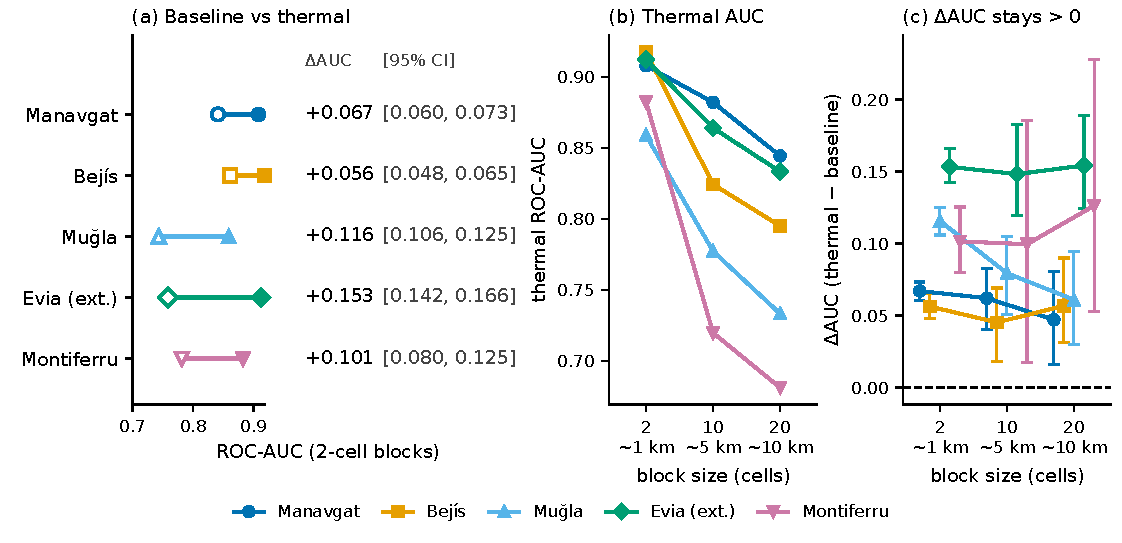
\includegraphics[width=140mm]{figures/fig3_within_robustness.pdf}}
  \caption{\textbf{The thermal increment replicates in all five regions and
  survives coarser spatial blocking.} Natural-vegetation primary population;
  random forest with the primary weighted configuration; all intervals are
  95\% spatial-block bootstrap intervals (1000 replicates, seed 42).
  \textbf{(a)} Baseline versus thermal out-of-fold ROC-AUC per region at the
  default 2-cell ($\sim$1\,km) blocking: the open marker is the static baseline
  feature set, the filled marker is the baseline plus the six thermal
  predictors, and the connecting bar is the increment. The right-hand column
  reports the paired $\Delta$AUC and its 95\% interval; it is a fixed column
  placed beyond the plotted AUC range, so no label position depends on a data
  value. Every interval excludes zero. \textbf{(b)} Absolute thermal ROC-AUC
  against spatial block size (2, 10 and 20 cells, $\approx$1, 5 and 10\,km):
  absolute skill falls as blocking coarsens, in every region.
  \textbf{(c)} The thermal increment $\Delta$AUC against the same block sizes,
  with 95\% intervals: the increment does \emph{not} melt away, and its
  interval excludes zero in all ten of the 2- and 10-cell region--block-size
  combinations. The five 20-cell intervals also lie above zero but rest on 6 to
  33 positive-carrying blocks each, so they are plotted as indicative rather
  than as intervals (Table~\ref{tab:1}, table note). In (c)
  the five regions are offset horizontally by 0.15 cell so their whiskers
  separate; \textbf{this offset is cosmetic, since all five regions are evaluated
  at exactly the same three block sizes} (2, 10, 20 cells), and the offset is
  smaller than half the spacing between block sizes, so the groups cannot
  merge. Colour and marker shape both encode region, so the panels remain
  readable in greyscale.}
  \label{fig:within-robustness}
\end{figure}

\begin{table}[htbp]
  \centering
  \small
  \caption{Within-region baseline versus thermal performance and block-size robustness. Primary (TSG) population; spatially blocked 5-fold CV (Section~\ref{sec:3.7}); paired spatial-block bootstrap, 1000 replicates. Block sizes 2/10/20 cells $\approx$ 1/5/10 km. Baseline and Thermal columns are ROC-AUC; the 95 \% CI belongs to $\Delta$AUC.}
  \label{tab:1}
  \begin{tabularx}{\linewidth}{>{\raggedright\arraybackslash}Xlllll}
    \hline
    Region & Block & Baseline & Thermal & $\Delta$AUC & 95\% CI \\
    \hline
    Manavgat 2021 & 2 & 0.841 & 0.908 & +0.067 & [+0.060, +0.073] \\
     & 10 & 0.820 & 0.882 & +0.062 & [+0.040, +0.082] \\
     & 20 & 0.798 & 0.845 & +0.047 & [+0.016, +0.081] \\
    Bejís 2022 & 2 & 0.862 & 0.918 & +0.056 & [+0.048, +0.065] \\
     & 10 & 0.779 & 0.824 & +0.045 & [+0.018, +0.069] \\
     & 20 & 0.739 & 0.795 & +0.057 & [+0.031, +0.090] \\
    Muğla 2021 & 2 & 0.743 & 0.859 & +0.116 & [+0.106, +0.125] \\
     & 10 & 0.698 & 0.777 & +0.079 & [+0.050, +0.105] \\
     & 20 & 0.673 & 0.733 & +0.061 & [+0.030, +0.094] \\
    North Evia 2021 (ext.) & 2 & 0.759 & 0.912 & +0.153 & [+0.142, +0.166] \\
     & 10 & 0.716 & 0.864 & +0.148 & [+0.119, +0.182] \\
     & 20 & 0.679 & 0.833 & +0.154 & [+0.124, +0.189] \\
    Montiferru 2021 & 2 & 0.781 & 0.883 & +0.101 & [+0.080, +0.125] \\
     & 10 & 0.620 & 0.720 & +0.099 & [+0.017, +0.186] \\
     & 20 & 0.555 & 0.681 & +0.126 & [+0.053, +0.228] \\
    \hline
  \end{tabularx}
\end{table}

\emph{Table note (resampling units).} The bootstrap resamples spatial blocks. An interval's reliability is therefore bounded by the number of blocks carrying at least one burned cell. Those counts fall from 192 to 843 at 2 cells to \textbf{6 to 33} at 20 cells. An interval built on six such blocks has no meaningful coverage, so \textbf{the 20-cell row should be read as indicative rather than as an interval}. The 10-cell row is the coarsest blocking this design supports properly. Every region there has 16 to 70 positive-carrying blocks, and the increment holds at that scale in all five regions (Appendix A(c)).

The Manavgat rows are computed on the corrected label. It adds burned cells, 784 to 2,935 in the primary population, and changes no predictor (Section~\ref{sec:3.2}). The rows strengthen rather than weaken. Absolute AUCs rise by 0.04 to 0.11 across the three block sizes, and the increment holds at every scale. The 1 km interval narrows from [+0.055, +0.079] to [+0.060, +0.073], because the region now carries 814 positive-carrying 2-cell blocks rather than 235.

This within-region result is not itself novel. It is reported because the transfer arms below are measured against it.

\subsection{What the evaluation frame is worth, within one region}\label{sec:4.3}

This section isolates the effect Section~\ref{sec:4.4} applies between regions. It comes first because it is measured on one model in one region with no transfer involved. Nothing the transfer arms do can therefore explain it (Appendix A(i)).

\textbf{Where the skill is lost, on a matched comparison.} Four evaluations are reported. The last three are scored on \textbf{identical cells}, so they differ only in what the model was trained on. The first shows why an unmatched comparison misleads. The held-out unit is a burned connected component of at least 50 cells, with all cells within 2 km of it. What makes that harder than a whole region is the composition of its negatives, not its burned fraction, and that is measured rather than argued. The same predictions were scored on a random sample of region cells drawn at the scar area's own burned fraction. That gives \textbf{0.793 against the region-wide 0.791}, so matching prevalence changes nothing, at $-$0.002 [$-$0.005, +0.001]. Scoring them on the scar area gives 0.644, a fall of \textbf{+0.149 [+0.087, +0.211]}. That swaps both pools at once, so each was swapped singly. Replacing only the negatives costs \textbf{0.139 [0.098, 0.181]}, the whole of it. Replacing only the positives costs \textbf{$-$0.002 [$-$0.055, +0.051]}, null on average, though the per-scar effect runs from $-$0.12 to +0.14. \textbf{The effect is the negative pool.} Every negative in a scar collar is fire-adjacent and shares the terrain, land cover and synoptic conditions of the positives, whereas a region's negatives include its easy far field. ROC-AUC is in any case invariant to class balance at fixed class-conditional distributions (\texttt{pool\_\allowbreak{}decomposition.\allowbreak{}json}).

\begin{table}[htbp]
  \centering
  \footnotesize
  \caption{The four evaluations, scored on identical cells. Primary natural-vegetation population. Rows B, C and D are scored on the held-out scar area; row A is the whole region and is shown to make the mismatch visible. Means and Student \emph{t} intervals are over the seven held-out scars.}
  \label{tab:2}
  \begin{tabularx}{\linewidth}{>{\raggedright\arraybackslash}X>{\raggedright\arraybackslash}Xlrl}
    \hline
    Evaluation & Model trained on & Scored on & Mean AUC & 95 \% CI \\
    \hline
    A. Blocked cross-validation, 5 km & the region, scar included & the whole region & 0.773 & [0.729, 0.818] \\
    B. Same blocked model, restricted & the region, \textbf{scar included} & the scar area & 0.640 & [0.544, 0.736] \\
    C. Leave-one-scar-out & the region, \textbf{scar withheld} & the scar area & 0.546 & [0.488, 0.604] \\
    D. Foreign region & another region, 306 to 2,802 km & the scar area & 0.553 & [0.495, 0.611] \\
    \hline
  \end{tabularx}
\end{table}

All four rows are means over the \textbf{same seven scars}. Bejís and Manavgat have no row C, because in each the burned area is a single component, so withholding it leaves nothing to train on. Under the corrected label the 2,151 added Manavgat burns merge into its one existing scar (2,934 of 2,935 cells). That is why the controls above are computed on nine scars and report 0.791 and 0.644 against this table's 0.773 and 0.640. The intervals are Student \emph{t} over the scars. That is this arm's resampling unit, rather than the spatial-block bootstrap used elsewhere. Four scars are in Muğla, two in Montiferru and one in Evia. \textbf{Row A is a region-level quantity repeated identically across a region's scars, so its interval is pseudo-replicated and should not be read as coverage.} That repetition propagates into A $-$ B and A $-$ C. Clustering by region, over three regions, gives \textbf{+0.137 [+0.048, +0.226]} and \textbf{+0.266 [$-$0.022, +0.553]}. The first still excludes zero. The second no longer does, and is 3.6 times wider. \textbf{The scar-level intervals on these two differences therefore overstate precision, and on the region unit only the frame cost is established} (Appendix A(i)).

\textbf{The same model, scored two ways on the same region, differs by 0.133 AUC.} Rows A and B are one model and one set of out-of-fold predictions. The only change is which cells they are scored on. That change alone costs \textbf{0.133 [+0.059, +0.207]} of the 0.227 [+0.147, +0.308] fall from A to C, about three fifths. That is a ratio of two estimates, so the point is the size of the numerator rather than the precision of the fraction. It is the size of the predictor-block increments this design itself measures. A region-wide blocked figure is therefore an upper bound on what the same model achieves where the fire actually is.

\textbf{Neither withholding the fire nor moving 2,800 km has a measurable cost.} B minus C, the fire-specific residual on identical cells, is \textbf{+0.094 [$-$0.012, +0.200]}. C minus D, the effect of replacing a same-region model with one fitted 306 to 2,802 km away, is \textbf{$-$0.007 [$-$0.070, +0.057]}. Both span zero and both arms sit close to chance. \textbf{With seven scars, two of them starved of positives, this design cannot establish a fire-specific residual, only bound it at about 0.20.} It is not shown to be zero on an unseen fire; what this design establishes is that it is not established there. Nor does it establish the fire \emph{event} as the unit, since the held-out patch is defined by the labels and its identity cannot be separated from its location. Appendix A(z) reports the spread behind row D, and the sweeps showing that the patch definition does not drive the result.

\textbf{The increment declines with the holdout, and is not established once the fire is withheld.} Contribution 2 concerns the paired thermal-minus-baseline difference, so the same evaluations were run on it. It is +0.056 to +0.153 under blocked cross-validation, with every interval above zero. It is +0.028 on a within-region half-split, \textbf{+0.024 [$-$0.040, +0.089]} under leave-one-scar-out, and +0.007 [$-$0.021, +0.037] across regions. The point estimate falls monotonically as the holdout hardens, and the last two intervals span zero. \textbf{The within-region increment is therefore substantially a property of interleaved holdout}.

\subsection{The same effect between regions, applied to our own matrix}\label{sec:4.4}

Section~\ref{sec:4.3}'s effect applies with equal force between regions. This test is reported before the transfer matrix because it changes what Section~\ref{sec:4.5} and Appendix A(s) can claim. It withdraws nothing in Section~\ref{sec:4.3}, which is what it is built from. Sources are \texttt{aoi\_\allowbreak{}frame\_\allowbreak{}auc\_\allowbreak{}frozen\_\allowbreak{}mugla.\allowbreak{}csv} and \texttt{aoi\_\allowbreak{}frame\_\allowbreak{}transfer\_\allowbreak{}frozen\_\allowbreak{}mugla.\allowbreak{}csv}, which supersede the pre-correction files for the reason given below, with \texttt{collar\_\allowbreak{}frame\_\allowbreak{}bootstrap.\allowbreak{}csv} and \texttt{diagnostics\_\allowbreak{}collar\_\allowbreak{}frame.\allowbreak{}csv}. Code is under \texttt{paper/\allowbreak{}code/\allowbreak{}}, and the elaboration is in Appendix A(w).

\textbf{The five areas of interest are not comparable frames.} Each is a rectangle drawn around a fire, and they differ by an order of magnitude in how much unburnt far field they enclose. The share of modelled cells beyond 10 km of any burned cell runs from \textbf{2.1 \%} in Montiferru to \textbf{63.1 \%} in Bejís (Appendix B, Table B6). That far field is not neutral. In Manavgat the median elevation of modelled cells rises from 330 m within 5 km of the fire to 1,273 m at 20 to 50 km, against 287 m for the burned cells themselves.

\textbf{Under an equalised frame four regions agree, and Manavgat does not.} Restricting every region to cells within 10 km of any burned cell removes only far-field negatives. Every burned cell is at distance zero and is retained at any radius, so the protection against a flattering radius is the sweep, not the retention of positives. On that frame the other four regions agree in sign on elevation, LST and TVDI, and Manavgat sits on the other side of 0.5 on all three. Its elevation reversal survives with support: 0.376 [0.300, 0.465] against Muğla's 0.606 [0.525, 0.685] and Evia's 0.648 [0.550, 0.740]. Under this paper's own criterion from Section~\ref{sec:3.10}, \textbf{two between-region reversals therefore remain bootstrap-supported under the collar}, both on elevation and both involving Manavgat. Its thermal channels move toward 0.5 without reversing with support (current LST 0.522 [0.451, 0.591]). At the point estimate, elevation, the three LST channels, TVDI and the two internally differenced channels therefore all straddle 0.5. The weaker difference instrument that Table B3's note commits this paper to supports three opposite-sided pairs on \texttt{lst\_\allowbreak{}anomaly\_\allowbreak{}mean}, with the caveats that keep it weak. \textbf{The honest statement is that the collar removes every elevation reversal except Manavgat's, which it leaves supported.} Two scope limits belong with it, both in Appendix A(l) and A(w). First, the interval criterion was evaluated at the 10 km collar only, though at the point estimate the 5 and 10 km radii agree. Second, the collar reduces two regions' cell counts substantially, so part of any loss of support is a loss of power. Features supported in both regions of a direction average 2.3 per direction on the full frame and 2.2 on the collar.

\textbf{The sign most regions share is not the one the dryness framing predicts.} At the point estimates a hotter pre-fire surface burned \emph{less} in four of five regions. On mutual adjustment temperature survives where greenness does not, so the absolute channels behave there as static land-surface descriptors rather than as dryness. Manavgat is the exception. Its burned cells are hotter (current LST 0.665 on the full frame), and they are also low-lying. Within distance to the nearest burned cell its LST signal falls to 0.454, so the thermal sign there cannot be separated from its terrain gradient. In Montiferru the signal is attenuated to near-null. The stratifications, the correlations and the reciprocal adjustment are in Appendix A(k). Section~\ref{sec:5.4} takes up what Manavgat's position may mean.

\textbf{The same test weakens a result of our own, but no longer dissolves it.} Under the frozen label, the diagnostic that best ordered transfer in our matrix reached $\rho$ = +0.84. That diagnostic is the sign-agreement fraction over interval-supported features. It is built from exactly these signed AUCs and was correlated against transfer on the same unequal frames. Under the corrected label it no longer orders transfer on the frames as drawn ($\rho$ = +0.52 [$-$0.27, +0.87]; Appendix D). Recomputed under the collar it is no longer degenerate. It takes the values 0 and 1 across sixteen defined directions and correlates with collar transfer at $\rho$ = +0.38 (p = 0.15), and its cosine variant at +0.40 (p = 0.12). The correction that once made it unanimous now leaves it weak on both frames (\texttt{diagnostics\_\allowbreak{}collar\_\allowbreak{}frame.\allowbreak{}csv}, \texttt{collar\_\allowbreak{}increment\_\allowbreak{}and\_\allowbreak{}cosine.\allowbreak{}csv}).

\textbf{Two further arms move with the frame.} The same-geography arm is the most extreme case in the cohort. A fixed study area is not a fixed evaluation frame, and its 2022 arm has 93.2 \% of cells beyond 10 km of any burned cell, against 55.3 \% for 2021. Under the collar its two arms therefore fall on the same side of 0.5 on elevation, the feature whose reversal we had reported for Muğla. The claim is scoped. That arm is reconstructed from the 2021 predictors, which are valid for the year-invariant channels and \textbf{not} the seasonal ones. \textbf{Only elevation and slope therefore carry a verdict, on both the Muğla reversal is removed, and on the thermal channels the arm is silent.} It rests on eleven positive-carrying blocks against a floor of sixteen (Appendices A(m), A(o)). The within-region increment, by contrast, \textbf{survives}, positive in all five regions at a mean of +0.083 against +0.087 as drawn.

\textbf{The transfer matrix moves as well.} Restricting source and target to the same collar:

\begin{table}[htbp]
  \centering
  \scriptsize
  \caption{Cross-region transfer under equalised evaluation frames. Primary natural-vegetation population, thermal model, twenty ordered directions per row. Above/below chance are point counts. The supported counts use a 10-cell ($\approx$5 km) spatial-block bootstrap on the target, 1000 replicates, seed 42. \textbf{Table B9 reports the same matrix under 2-cell ($\approx$1 km) blocking}, which is why its supported counts are the larger 11 and 7 (Section~\ref{sec:4.5}). Per-direction bounds are in \texttt{aoi\_\allowbreak{}frame\_\allowbreak{}transfer\_\allowbreak{}frozen\_\allowbreak{}mugla.\allowbreak{}csv}.}
  \label{tab:3}
  \resizebox{\ifdim\width>\linewidth\linewidth\else\width\fi}{!}{%
  \begin{tabular}{llrrrrr}
    \hline
    Source frame & Target frame & Mean target AUC & Above chance & Below chance & Supported above / below & Paired thermal delta \\
    \hline
    full & full (\textbf{Table B9}) & 0.527 & 13 of 20 & \textbf{7} & 9 / \textbf{6} & +0.007 \\
    full & 10 km & 0.559 & 14 of 20 & 6 & 10 / 2 & +0.008 \\
    10 km & full & 0.546 & 14 of 20 & 6 & 10 / 5 & +0.014 \\
    \textbf{10 km} & \textbf{10 km} & \textbf{0.589} & \textbf{15 of 20} & \textbf{5} & \textbf{13 / 2} & \textbf{+0.024} \\
    5 km & 5 km & 0.591 & 16 of 20 & 4 & 11 / 0 & +0.017 \\
    \hline
  \end{tabular}}
\end{table}

\textbf{A data-provenance defect in this arm was found and corrected.} One region's predictor file at the canonical path had come to differ from the one the frozen tables were computed on, so every arm here was re-run against the frozen export. The correction moves forty of a hundred per-direction values by up to 0.022. It leaves \textbf{every headline quantity above unchanged to within 0.0012}, and the signed AUCs of that region's two channels move by at most 0.008, with no verdict changing (Appendix A(w)). The table reports the corrected values, and reproduces Table B9's as-drawn mean of 0.527 and 13 of

\begin{enumerate}
  \item \textbf{The baseline control must be restated on this frame.} The static baseline transfers at 0.565
\end{enumerate}
against 0.589, a paired difference of +0.024 rather than +0.007. The control therefore holds in kind, but the gap is about three times larger once frames are comparable, and about twice as large at the 5 km collar.

\textbf{What this settles, and what it leaves standing.} Four quantities reported below are properties of the frames rather than of the predictor-burning relationship, and are identified as such where they appear. They are the count of below-chance directions, which falls from seven to five; the sign-agreement diagnostic; the same-geography arm; and the paired thermal contribution, +0.007 as drawn against +0.024 equalised. One is not: Manavgat's elevation reversal, which the collar leaves supported. The paired contribution carries the portability null, so it is given an interval on the frame this section argues for: \textbf{+0.024 [$-$0.004, +0.049]} under the pair-cluster resampling of Appendix A(o). It still spans zero, so the null survives the correction, but only just. Under the alternative admissible unit, clustering by target region, it does not ([+0.011, +0.040]; Appendix A(w)). What survives is the central negative result, and its size must be stated on a matched comparison. Setting 0.589 against a within-region reference of about 0.90 would compare a collar number with a full-rectangle one at 1 km blocking. Recomputed on the same frame at 5 km blocking, that reference is 0.786. The shortfall is therefore \textbf{+0.197 [+0.091, +0.303]}, a Student \emph{t} interval over the five target regions rather than the spatial-block bootstrap used elsewhere. Manavgat contributes the largest per-region shortfall to it (+0.319; Appendix A(w)). The shortfall is real, and it is 0.197 rather than the 0.29 an unmatched comparison implies. Appendix C.5(ix) records the frame as a limitation of this cohort rather than of the method.

\subsection{Cross-region transfer, and what label-free adaptation does to it}\label{sec:4.5}

\textbf{Everything in this section is computed on the frames as drawn and should be read against Section~\ref{sec:4.4}.} That section has shown the frames are not comparable, and that the within-region reference used here is itself frame-dependent. The as-drawn matrix is reported because it is what the original analysis protocol yields. Per-direction values are in Appendix B, Table B9, and the supporting arms in Appendix A(ix).

\textbf{Raw transfer is heterogeneous and includes anti-predictive directions.} Target AUC spans 0.314 to 0.677, and Fig.~\ref{fig:transfer-matrix} gives the matrix direction by direction. The support counts depend on the blocking scale, so both are reported. At 2-cell ($\approx$1 km) blocking, eleven of twenty directions are above chance with interval support and seven below. At the 10-cell ($\approx$5 km) blocking this design defends, nine are above and six below with five uncertain; these are the counts Table~\ref{tab:3} uses. Of the below-chance directions, two keep interval support after frame equalisation, Manavgat to Bejís and Muğla to Manavgat. Across five bootstrap seeds every 2-cell verdict is stable. At 10 cells, one level verdict and two paired-delta verdicts are not (\texttt{transfer\_\allowbreak{}ci\_\allowbreak{}blocksize.\allowbreak{}csv}). Even the best raw transfer sits far below the target's own within-region skill: Evia to Manavgat reaches 0.677 against Manavgat's 0.908. The raw deficit runs from 0.231 to 0.594, against a reference that Section~\ref{sec:4.3} shows is not matched to a transfer evaluation.

\begin{figure}[htbp]
  \centering
  \makebox[\linewidth][c]{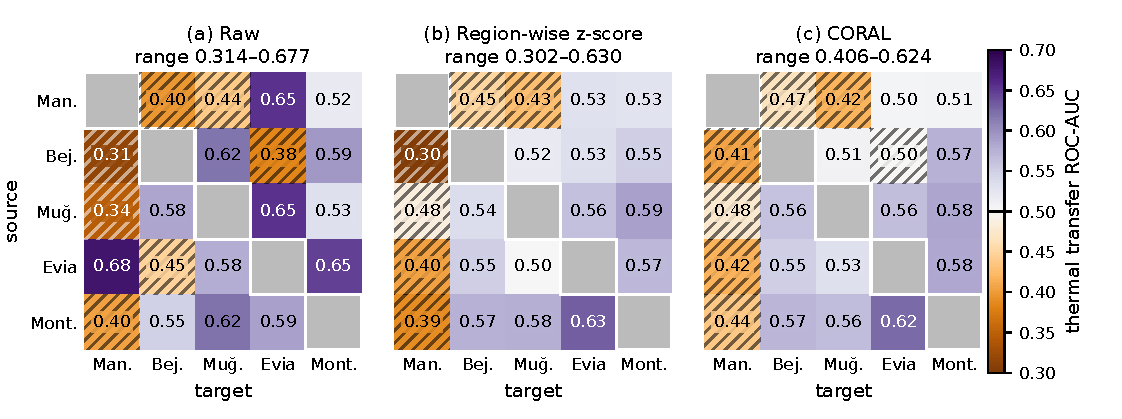
\includegraphics[width=140mm]{figures/fig4_transfer_matrix.pdf}}
  \caption{\textbf{Cross-region transfer, and what label-blind adaptation does
  to it.} Thermal transfer ROC-AUC for all 20 ordered source--target
  directions among the five regions, natural-vegetation primary population.
  \textbf{(a)} Raw transfer, no adaptation. \textbf{(b)} After region-wise
  z-score standardisation. \textbf{(c)} After CORAL. Rows are the source
  region, columns the target; the grey diagonal is within-region performance
  and is \emph{not} a transfer result. The diverging colour scale is centred
  exactly on chance (0.5, marked by the black rule on the colour bar), so
  orange is below chance and purple above. Each panel header states that
  panel's range: adaptation narrows the spread from 0.314--0.677 (raw) to
  0.302--0.630 (z-score) and 0.406--0.624 (CORAL). It compresses the matrix
  toward chance rather than lifting transfer, with one exception at the low end:
  under z-scoring Bej\'is$\rightarrow$Manavgat moves further below chance
  (0.314 to 0.302). Cells below chance are hatched.
  The hatch is a redundant cue for print: a diverging palette is symmetric in
  luminance about its centre, so in greyscale a below-chance cell would
  otherwise be indistinguishable from an equally distant above-chance one.
  Hatching follows the \emph{exact} value while the printed label is rounded to
  two decimals, so three cells print ``0.50'' with different hatching: CORAL
  Bej\'is$\rightarrow$Evia is 0.4991 (hatched, below chance), while z-score
  Evia$\rightarrow$Mu\u{g}la is 0.5013 and CORAL Manavgat$\rightarrow$Evia
  0.5043 (both un-hatched, above chance). Every cell carries its value, and
  every label's colour is chosen by measured WCAG contrast against that cell's
  rendered colour (worst case 4.6:1). Confidence intervals for these directions
  are given in Table~B9. Manavgat directions are on the corrected label
  (Section~\ref{sec:3.2}).}
  \label{fig:transfer-matrix}
\end{figure}

\textbf{Manavgat is the weakest target in the matrix}, at a mean of 0.435 over its four incoming directions against 0.494 to 0.572 for the other targets. It is not the weakest source (0.502, against 0.477 for Bejís). Three of its incoming directions lie between 0.314 and 0.404, while Evia to Manavgat reaches 0.677. An exploratory split by fire phase suggests where the collapse sits; it was not registered, and it concerns one region and one event. The corrected label's added cells burned on 28--31 July, the fire's first four days, and the remaining 784 later. Transfer into the early cells is lower than into the later ones in every direction: Bejís 0.276 against 0.419, Montiferru 0.351 against 0.549, Muğla 0.332 against 0.382, and Evia 0.667 against 0.704. The early cells also lie far lower, at a median of 219 m against 512 m for the later burns and 1,004 m for unburned cells (\texttt{paper/\allowbreak{}labelfix\_\allowbreak{}rerun/\allowbreak{}round5/\allowbreak{}s4b\_\allowbreak{}*}). Section~\ref{sec:5.4} treats this as a mechanism proposal, not as evidence.

\textbf{In precision terms it is worse than the ROC figures suggest.} A susceptibility surface is used as a ranked area budget, so precision-recall is the operational quantity. PR-AUC averages \textbf{0.181 against a no-skill baseline of 0.157}. \textbf{Seven of twenty directions fall below their own baseline at the point estimate, all seven with intervals entirely below it.} Only one direction, Evia to Manavgat, exceeds twice its baseline. These are frame-as-drawn quantities, and the PR arm was not recomputed on the collar (Appendix B, Table B4).

\textbf{The static baseline does not transfer either}, at a mean of \textbf{0.519} against \textbf{0.527} for the thermal model. The failure is therefore not specific to the dynamic block. A baseline that does not travel, plus pre-fire thermal state, gives a model that does not travel. Section~\ref{sec:4.4} restates this control on the equalised frame, where it is 0.565 against 0.589.

\textbf{The thermal block's paired contribution is +0.007, and the mean is not the informative statistic.} The individual contributions span \textbf{$-$0.148 to +0.133}, twelve positive and eight negative. The largest is about twenty times the mean, and the sign belongs to the pair rather than to the block. A mean near zero records cancellation, not consistent absence of effect. The directions are not independent, since each region appears in eight of the twenty, so the interval depends on the resampling unit. \textbf{All four units the design permits give the same answer}, from [$-$0.018, +0.033] to [$-$0.028, +0.045], and none propagates within-direction sampling variability. The leave-one-region-out jackknife shows the mean is not carried by any single region. Dropping one region at a time moves it between +0.001 (without Evia) and +0.015 (without Manavgat), and never reverses its sign.

\textbf{Label-blind adaptation compresses the matrix toward chance rather than repairing it} (Fig.~\ref{fig:adaptation}). Under region-wise z-scoring the twenty directions span 0.302 to 0.630, and under CORAL 0.406 to 0.624. Sixteen of twenty move closer to chance, which helps the directions that failed and harms those that worked. The committed-in-advance CORAL arm averages \textbf{0.517}. Taking whichever method scores better per direction gives 0.523, but that selection uses the target labels the protocol forbids. It is therefore \textbf{an oracle upper bound rather than an achievable result}. Even the oracle stays below the reference a model reaches on an unseen scar (Section~\ref{sec:4.3}, row C, 0.546). Alignment is thus regressing the matrix toward that reference rather than exceeding it. A sign reversal is not a distribution mismatch that realigning inputs would repair. Appendix A(ix) reports the recovery fractions, including the seven directions with \emph{negative} recovery.

\begin{figure}[htbp]
  \centering
  \makebox[\linewidth][c]{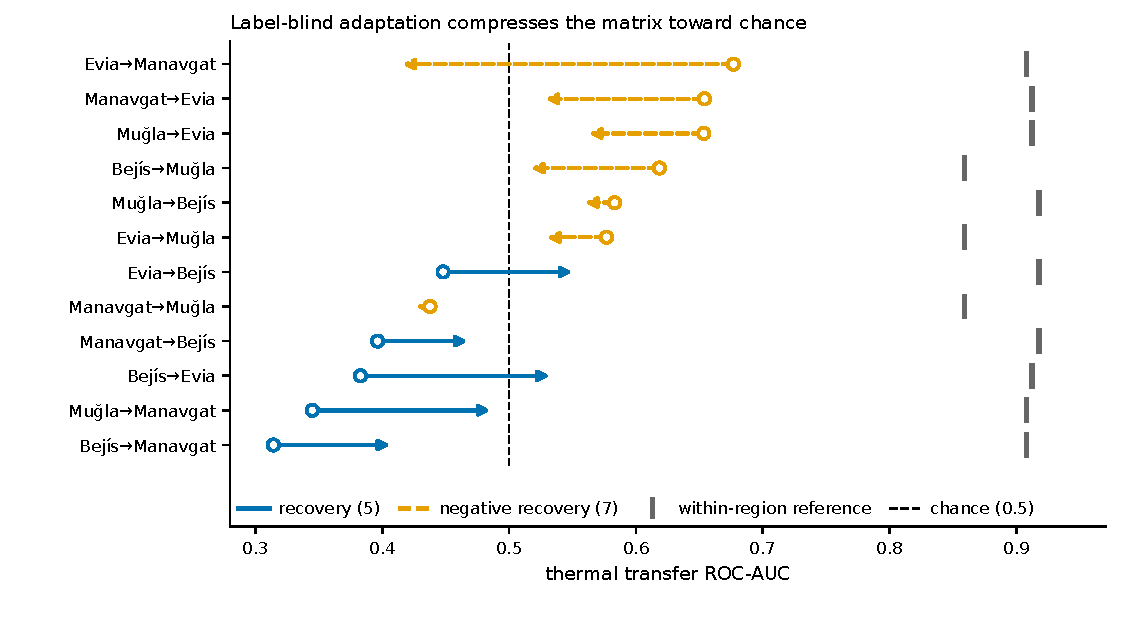
\includegraphics[width=140mm]{figures/fig5_adaptation.pdf}}
  \caption{\textbf{Label-blind adaptation regresses transfer onto the level a
  model reaches on an unseen scar, rather than recovering it.} All 12 ordered directions among the
  four regions carrying the full decomposition (Manavgat, Bej\'is, Mu\u{g}la,
  Evia), natural-vegetation primary population. Each row is one direction. The
  open circle is raw transfer ROC-AUC and the arrow runs to the best
  label-blind adapted result for that direction (region-wise z-score or CORAL,
  whichever is better); the grey vertical tick is the within-region reference
  for that target, and the dashed vertical rule is chance. \textbf{Solid blue
  arrows are the five directions where adaptation moves transfer toward the
  within-region reference (recovery); dashed orange arrows are the seven where
  it moves \emph{away} from it (negative recovery).} Line style and colour both
  encode this class, because the two hues differ by only 2.30:1 in relative
  luminance and would nearly merge in greyscale. The pattern is the point: all
  six directions starting above chance are pushed down, and five of the six
  starting below chance are pushed up, so adaptation acts on the spread rather
  than on skill. The exception is Manavgat$\rightarrow$Mu\u{g}la, which starts
  below chance at 0.470 and is pushed further down to 0.443. The worst case is Evia$\rightarrow$Manavgat, where raw transfer of
  0.686 is dragged down to 0.527 against a within-region reference of 0.870, a
  recovered fraction of $-0.862$. No arrow reaches its within-region tick.}
  \label{fig:adaptation}
\end{figure}

\subsection{Further arms}\label{sec:4.6}

Six further arms bear on the findings above without changing them. They are the contrast pair (A(s), Fig.~\ref{fig:contrast-pairs}), the two interventions (A(n)), the sensitivity summary (A(v)), the same-geography two-event arm (A(m)), the distance curve (A(t)) and the label-budget curve (A(u)). Each is stated there with its own limits. Two are plotted here because the shape of the result is the argument. Pooling every other region does not beat the best single source for four of five targets; for Evia the pooled model exceeds it (0.715 [0.668, 0.757] against 0.654; Fig.~\ref{fig:loro}). Removing the direction-reversing features costs within-region skill and returns nothing measurable on transfer (Fig.~\ref{fig:feature-drop}).

\begin{figure}[htbp]
  \centering
  \makebox[\linewidth][c]{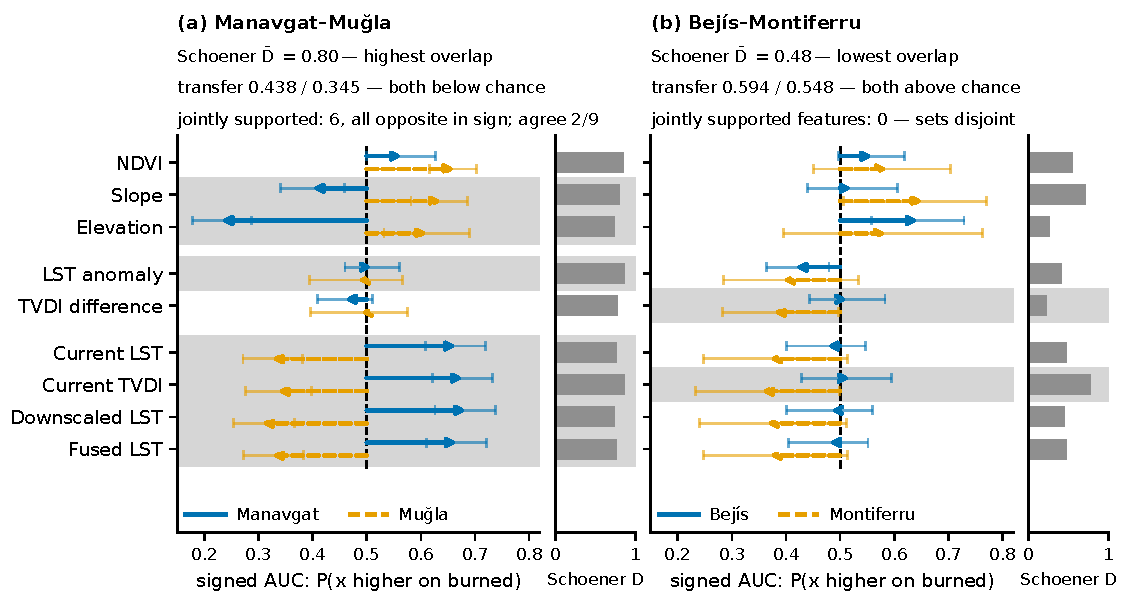
\includegraphics[width=140mm]{figures/fig8_contrast_pairs.pdf}}
  \caption{\textbf{The contrast pairs.} \textbf{(a)} Manavgat--Mu\u{g}la, the
  pair whose burned cells overlap most in environmental space (mean Schoener
  $\bar{D}=0.80$, rank 1 of 10 on all five overlap measures), transfers below
  chance in both directions at the point estimates (0.438 and 0.345).
  \textbf{(b)} Bej\'is--Montiferru, the pair that overlaps least
  ($\bar{D}=0.48$, rank 10), transfers above chance in both directions at the
  point estimates (0.594 and 0.548). Arrows run from 0.5 to each region's
  signed univariate AUC, the probability that a predictor takes a higher value
  on a burned cell than on an unburned one. A filled head marks a 95\%
  spatial-block (10-cell, $\approx$5\,km) bootstrap interval that excludes 0.5;
  an open head marks one that does not. Solid blue is the first region named,
  dashed orange the second; line style is included because the two hues nearly
  merge in greyscale. Shaded rows mark features whose sign differs between the
  two regions, and side bars give Schoener's $D$ per feature. In (a), six
  features are interval-supported in both regions, and all six have opposite
  signs; the signs agree on 2 of 9 features overall. In (b) the two supported
  sets do not intersect, and the signs agree on 7 of 9. The transfer verdicts use
  the 1\,km bootstrap, under which all four directions are off chance. At 5\,km
  blocking only Mu\u{g}la $\rightarrow$ Manavgat stays interval-supported, which
  is why the contrast is stated at the point estimates. Manavgat values are on
  the corrected label (Section~\ref{sec:3.2}).}
  \label{fig:contrast-pairs}
\end{figure}

\begin{figure}[htbp]
  \centering
  \makebox[\linewidth][c]{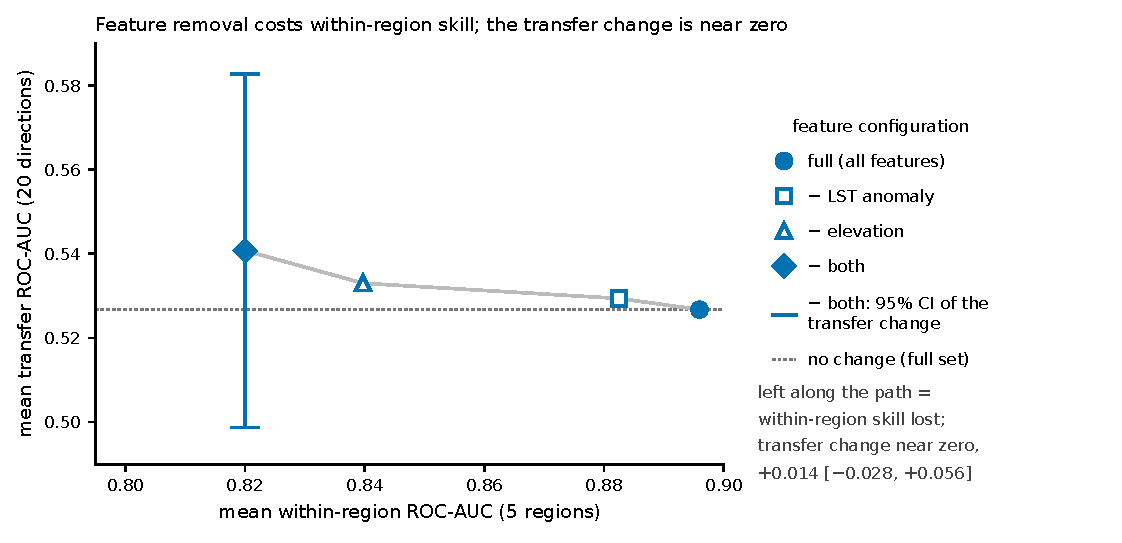
\includegraphics[width=140mm]{figures/fig7_feature_drop.pdf}}
  \caption{\textbf{Removing the direction-reversing features costs locally and
  returns nothing measurable on transfer.} Mean within-region ROC-AUC across the five regions (horizontal)
  against mean transfer ROC-AUC across the 20 ordered directions (vertical),
  for four feature configurations: the full thermal set, the set without the
  LST anomaly, without elevation, and without both. Each configuration has its
  own marker and is named in the key; the grey path connects them in that
  order. Moving left along the path, transfer rises monotonically
  (0.541 $\rightarrow$ 0.556) while within-region skill falls monotonically
  (0.888 $\rightarrow$ 0.807). Both monotonicities are verified when the
  figure is built, so the figure cannot silently contradict the claim. The
  within-region cost is 0.081 AUC and is supported in every region. The change
  in transfer is $+$0.014 AUC on an interval that spans zero, so no exchange
  between the two is demonstrated: a local cost is measured and no compensating
  transfer gain is.}
  \label{fig:feature-drop}
\end{figure}

\begin{figure}[htbp]
  \centering
  \makebox[\linewidth][c]{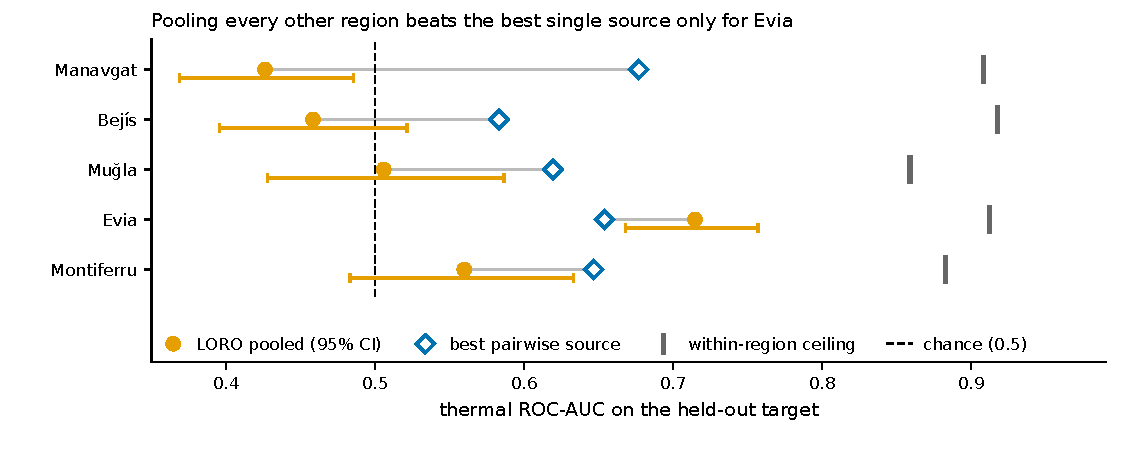
\includegraphics[width=140mm]{figures/fig6_loro.pdf}}
  \caption{\textbf{Pooling every other region does not beat the best single
  source for four of five targets.} Leave-one-region-out evaluation: for each held-out target region
  (rows), a model trained on the pooled remaining four regions (filled orange
  circle) is compared against the best individual source region for that same
  target (open blue diamond), with the within-region ceiling as a grey vertical
  tick and chance as the dashed rule. Natural-vegetation primary population,
  thermal feature set, no adaptation. The pooled model lies to the left of the best pairwise source in four
  targets. For Evia it lies to the right, at 0.715 [0.668, 0.757] against 0.654
  for the best single source, Manavgat (Section~\ref{sec:5.3}). Elsewhere, adding
  source regions does not accumulate transferable signal. In two targets the
  pooled model falls \emph{below chance} at the point estimate (Manavgat 0.426,
  Bej\'is 0.458), and only for Manavgat does the interval lie entirely below
  chance, while a single well-chosen source reaches 0.677 and 0.583
  respectively. Every point remains far below the within-region ceiling.
  Manavgat values are on the corrected label (Section~\ref{sec:3.2}).}
  \label{fig:loro}
\end{figure}

Two arms bear directly on Sections~\ref{sec:5.3} and \ref{sec:5.6}. The first is the interventions. There a local cost of $-$0.076 is measured against a transfer return of +0.014 [$-$0.028, +0.056], whose interval spans zero. The two removed features were fixed from the frozen label's supported reversals, and are kept, not re-selected. The second is the label budget. Thirty-two labelled 5 km blocks recover 83 to 89 \% of the target's matched ceiling in three of six directions, and 30 to 52 \% in the rest. Those blocks are 7 to 20 \% of the target's population, drawn from the event being predicted, which is not a resource available before that event burns.

No diagnostic among the twenty fixed in advance orders transfer with an interval excluding zero (Appendix D). One of them, the supported-feature vector Spearman, is defined on only six directions and was not evaluated as a diagnostic.



\section{Discussion}\label{sec:5}

\subsection{Reading the three findings together}\label{sec:5.1}

Section~\ref{sec:1.3} states the three findings and Section~\ref{sec:4} establishes them; this section argues from them. The relation between them is what makes the paper cohere. The first is not a caveat attached to the second; it is the instrument that sets its size. Applied to our own matrix, it identified four quantities as properties of the frames rather than of the relationship between predictors and burning. What it left standing is a shortfall in transferred skill and one reversed relationship, Manavgat's elevation. The third closes the obvious way around the second. If transfer cannot be assumed, it might still be anticipated from how similar two regions are, and no diagnostic in the set fixed in advance was shown to do that.

\subsection{Why the thermal increment is real but local}\label{sec:5.2}

The within-region increment and the transfer failure are measured at different separations, and Section~\ref{sec:4.3} shows most of the difference is already present inside a single region. The increment is local in a specific sense. It holds where held-out cells are interleaved with training cells, and most of it is gone once they are not, before the fire or the region changes. It is not an artefact to be explained away: it survives every sensitivity arm of Appendix A(a)--(h), and window closure stays positive and supported in all five regions on the corrected label. But it is established under interleaved validation and not beyond it. Even there the window-closure arm \textbf{weakens monotonically in Evia}, so what holds everywhere is survival, not improvement.

\textbf{That comparison is established at the scar, not at the region, and this weakens the claim.} Section~\ref{sec:4.3} measures the fall from a blocked within-region figure to an unseen scar over seven scars in three regions. Clustered by region, the frame cost stays clear of zero at +0.137 [+0.048, +0.226]. The whole fall to an unseen scar does not: it is +0.266 [$-$0.022, +0.553]. On the region as the unit, then, only the frame cost is established. The fall to an unseen scar is supported at the scar level only, and this cohort gives it no region-level support.

The natural objection is that Mediterranean regions are simply different systems, so a predictor meaning one thing in one place and another elsewhere compares two systems rather than showing instability. \textbf{We designed the two-Muğla-events arm to answer that objection and it does not answer it}: Section~\ref{sec:4.4} shows it is the most extreme frame artefact in the cohort. Three further confounds were never resolved in any case. Season and year \textbf{cannot be resolved in this study area}, the population is not fixed, and the positive-block count is below this design's own floor (Appendix C.5(ii)). With one fire per region everywhere else and that arm withdrawn, \textbf{this cohort provides no evidence that the transfer shortfall is regional rather than event-specific}. Appendix A(t) adds a length scale for the within-region decay but cannot turn it into an attribution either.

One conclusion survives from the other direction. The static baseline transfers no better than the dynamic block, at a mean of 0.519 against 0.527, so whatever the shortfall is, it is not the thermal block's peculiarity.

\subsection{What the two interventions do and do not show}\label{sec:5.3}

Both interventions show a similar shape, with one exception. Pooling four regions does not beat the best single-source transfer for four of five targets, and it stays well below the within-region ceiling for all five (Appendix A(n)). For Evia the pooled model exceeds the best single source, at 0.715 [0.668, 0.757] against 0.654. Manavgat's corrected label appears to carry conditional information for Evia, and it shows in two separate analyses: raw transfer from Manavgat to Evia rises from 0.613 to 0.654, and the pooled model that includes Manavgat reaches 0.715. Both use Manavgat as a source, so they are not independent confirmations. We record one observation about the pairing, as an observation and not as a return to the regime hypothesis of Section~\ref{sec:5.4}. The only target where pooling helps shares an event structure with one of its sources. Manavgat and Evia are the two fires in the cohort that burned as a single large scar, of 2,934 and 2,653 cells, in late July and early August 2021. Muğla burned in the same weeks but as ten separate scars, and Bejís burned as a single scar of 1,100 cells in 2022. Elsewhere pooling does not manufacture the missing conditional information. Removing the reversing predictors costs $-$0.076 of within-region skill with interval support in every region, and returns +0.014 [$-$0.028, +0.056] in mean transfer.

That pair of numbers is easy to read as an exchange, and it is not one. Both arms are null on the portability axis. The thermal block's own contribution is +0.007 and removal returns +0.014, both with intervals spanning zero, so they measure a local cost and no compensating gain. That is not a conservation law and not a rate at which local skill can be sold for portability; no such rate is estimated here.

\subsection{The regime hypothesis, reported as it happened}\label{sec:5.4}

A regime-structure explanation was stated in advance and the data confirmed the null. The regime-distance correlation has the wrong sign at the point estimate ($\rho$ = +0.109). The most regime-similar pair, Bejís and Manavgat, fails in both directions (0.396 and 0.314). The most regime-different pair, Bejís and Muğla, transfers above chance in both (0.618 and 0.583). One mundane explanation can be set aside: subsampling Muğla, much the largest population, to Manavgat's cell count leaves its transfer behaviour inside the subsampling range in both roles. The error was in the hypothesised grouping, not in the data, and with ten pairs this cannot refute regime typology \citep{Archibald2013} in general.

\textbf{Manavgat is where the matrix fails most, and three indicators point there.} It has the most outlying univariate profile in the cohort, with elevation at 0.232 and the three LST channels near 0.67, all interval-supported and all opposite to the other four regions. It also carries the largest matched shortfall (+0.319) and is the weakest target (0.435). The three point at the same region, and that is not a coincidence. A model trained where burned cells sit higher and cooler than their surroundings is asked to rank a fire that burned low and hot. The exploratory phase split of Section~\ref{sec:4.5} suggests where the collapse sits. The cells that burned in the fire's first four days lie at a median of 219 m, and their LST signal is the strongest in the region (AUC 0.70 to 0.72 with interval support, against 0.57 to 0.58 later). Transfer into these early cells is lower from every source, and the static baseline collapses there too. Elevation is reversed in both phases (0.197 and 0.328). With this data, elevation and temperature cannot be separated, because the low ground is also the hot ground.

We therefore offer a mechanism proposal, not a finding. The sign of elevation, and with it the sign of the thermal channels, may be set by which part of the elevation gradient an event burns relative to its frame, rather than by the region. Muğla shows the same pattern across its 2021 and 2022 events. The 2021 fire burned high relative to its frame (elevation AUC 0.611), the 2022 fire low (0.297), and the reversal is interval-supported inside a single study area. The link has a limit that belongs with it. Muğla's reversal is carried by the 2022 arm's far field and the collar removes it (0.606 against 0.565), whereas Manavgat's survives the collar (0.376). The two cases therefore share the pattern on the frames as drawn but differ in how much of it the frame explains. Testing the proposal needs several events per region spread along the elevation gradient, and predictors that separate terrain from surface temperature.

\textbf{Measures built from interval support carry a warning for future work.} Measures that count or weight only interval-supported features are structurally sensitive to flags on a knife edge. Under both labels, five to six of the pipeline's interval bounds lie within 0.01 of 0.5. A single such flag, Manavgat's NDVI, moved the full-frame supported-feature cosine from $\rho$ = 0.49 to 0.70 when two equally valid bootstrap streams disagreed on it. A threshold on the interval turns small shifts in the inputs into discrete changes in the feature set. This partly explains why the conditional-similarity result fell from +0.84 to +0.52 [$-$0.27, +0.87] under the corrected label. Work that uses such measures should report how many bounds lie near the threshold, and should repeat the calculation across bootstrap streams before reading a correlation.

\subsection{The empirical contrast with Dimarco et al.}\label{sec:5.5}

\citet{Dimarco2026} transfer successfully across a comparable Mediterranean design and we do not, and the two results are not in conflict. Their predictors are attributes of a place, ours the state of a surface in one season. That suggests the relation between domain similarity and transfer success depends on the predictor class.

That reading is one of at least two, and we cannot separate them here. Their response variable is human-driven \textbf{ignition}, dominated by access and activity, while ours is burned \textbf{area}, dominated by spread. A predictor-class explanation and a response-variable explanation are therefore confounded in this comparison. Our own data speak against a simple predictor-class reading in any case: the static baseline transfers at a mean of 0.519 here, so within this cohort the place-attribute class does not travel either.

\subsection{Implications}\label{sec:5.6}

In precision-recall terms, which is how a susceptibility surface is used, transferred models average a PR-AUC of 0.181 against a no-skill baseline of 0.157 \textbf{on the frames as drawn}. Seven of twenty fall below their own baseline, all seven with intervals entirely below it (Section~\ref{sec:4.5}). Whatever the ROC figures suggest, a model moved to a region it was not fitted in does not usefully rank burned cells there.

The paper supports one concrete change in reporting: alongside a spatially blocked within-region figure, report skill on a held-out burn scar and its surroundings. On these five regions the two differ by about 0.13 ROC-AUC on the same model, the size of the effect such papers usually claim, and this frame cost holds with the region as the unit (Section~\ref{sec:5.2}). \textbf{A blocked figure alone should therefore be read as an upper bound.} Transfer skill likewise has to be \emph{measured} on the target region rather than assumed from a within-region figure. Where a model must be moved, the resource that closes the gap is target labels (Appendix A(u)): a real answer, but not a cheap one.

The results also bound what unsupervised alignment can be asked to do. Even the oracle selection, which uses the target labels the protocol forbids, only reaches the reference a model can reach on an unseen scar (Section~\ref{sec:4.5}). Alignment is not failing far below an achievable target; it is regressing the matrix onto it, at the cost of the directions that already worked. A sign reversal is not a distribution mismatch that realigning inputs repairs.

\subsection{Limitations}\label{sec:5.7}

Appendix C.5 states the limitations in full, and seven bind the conclusions above. \textbf{The frames are not comparable and this cohort cannot fully repair it} (Section~\ref{sec:4.4}). The collar radius is itself a choice, with 5 km and 10 km giving 0.591 against 0.589, and the frames were fixed upstream, so we can restrict them but not extend them. Any future cohort should fix the frame by an explicit accessible-area rule \citep{Barve2011} before any predictor is computed; that is the main design lesson of this paper. \textbf{Each region contributes one fire season}, so regional concept shift is confounded with event meteorology and the shortfall cannot be attributed to region rather than event (Section~\ref{sec:5.2}). \textbf{The diagnostic correlations rest on an effective sample of ten region pairs}, so the diagnostic results of Appendix D, successes and failures alike, read at that power.

\textbf{The interval-support measures are less stable than the point estimates behind them.} Five to six interval bounds lie within 0.01 of 0.5, so one flag can move a diagnostic correlation by about 0.2 (Section~\ref{sec:5.4}). The transfer verdicts are steadier: at 2-cell blocking every verdict is stable across five bootstrap seeds, and at 10 cells one level verdict and two paired-delta verdicts are not.

\textbf{The phase split cannot separate elevation from temperature.} The cells that burned first are both the lowest and the hottest, so the proposal of Section~\ref{sec:5.4} is confounded in this data by construction. \textbf{It also rests on one region and one event.} The split was not registered, and it cannot be generalised until other events that burn across the elevation gradient are examined.

\textbf{The quality-screening comparison also changes the code.} The current pipeline's step7 refuses the unscreened MODIS input, so the unscreened arm uses the step7 of export time and the screened arm the current one. The two arms therefore differ in code version as well as in screening. They agree on elevation to four decimals and on every other signed AUC to within 0.005, so the confound could only have hidden an effect if two effects cancelled. It is stated because an earlier description of both arms as rebuilt was inaccurate.

The remaining six, from the absent meteorological covariates to the classifier comparison made by point estimate only (Appendix A(h)), bear on scope rather than on the conclusions above.



\section{Conclusions}\label{sec:6}

Where a fire model is scored decides what it appears to know. Model, predictors and fitting were held fixed, and only the scored cells changed. Moving from a whole study region to the burn scar and its 2 km collar costs \textbf{0.133 ROC-AUC}. A control measures the cause as the composition of the negative pool rather than class balance. That is the size of the predictor-block increments this design itself measures. A region-wide validation figure should therefore be read as an upper bound on what a model achieves where fire actually occurs, and reported as one.

That correction is not only other people's problem. Applied to our own five-region matrix, it shows four of our own quantities to be properties of the frames. The study areas enclose very unequal far fields. Equalising them to a 10 km collar lifts mean transfer from 0.527 to 0.589 and reduces the directions below chance. It removes every supported elevation reversal but one, Manavgat's, which survives. The same correction applies to the one arm that held place fixed, two fires in one study area eleven months apart. We had wrongly exempted it, because its geography was constant while its evaluation frame was not. Its elevation reversal does not survive equalisation, and that arm can speak only for the year-invariant channels. Much of what had looked like a reversed predictor-burning relationship was a statement about how five rectangles were drawn.

What survives is the central result. Pre-fire thermal predictors add a real and repeatable within-region increment in all five regions. It survives spatial blocking at about 5 km, and a predictor window closed up to two weeks before the first labelled burning. It does not travel. On matched frames and blocking, equalised transfer of 0.589 falls 0.197 short of the within-region reference. The paired cross-region contribution spans zero on both frames under the resampling unit we treat as primary, though not when clustered by target region (Section~\ref{sec:4.4}), and its sign varies by pair. The static baseline transfers no better on either frame, so this is not a peculiarity of thermal predictors. Label-free alignment compresses most directions towards chance rather than repairing them.

Two limits belong with all of this. The thermal direction shared by most regions is the opposite of the one the dryness framing predicts. Hotter pre-fire surfaces burned less in four of five regions, and holding greenness does not remove it, while holding temperature reverses greenness in two regions. On this cohort the absolute channels therefore behave as static land-surface descriptors rather than as a dryness index. Manavgat is the exception, and there its thermal sign cannot be separated from its terrain. And with one fire per region, and the single arm that held place fixed now withdrawn, this design measures a transfer shortfall but cannot attribute it to region rather than to event.

Three practical consequences follow. Report local skill and portability separately, since a predictor block worth a large within-region increment may contribute nothing distinguishable from zero across regions. Fix the evaluation frame by an explicit accessible-area rule before any predictor is computed, because a frame chosen for convenience can manufacture both a transfer failure and a mechanism to explain it. And do not screen for transfer by similarity. None of the twenty diagnostics fixed in advance was shown to order transfer. At the point estimates, the most similar pair failed in both directions while the least similar transferred above chance. Without labels from the target region, a model's skill there is unknown, and no measure computed beforehand stands in for it. With them, skill can be measured and the model recalibrated, but the price depends on the direction. Thirty-two labelled 5 km blocks recover 83 to 89 \% of the target's matched ceiling in three of six directions, and only 30 to 52 \% in the other three (Appendix A(u)). Those labels came from the event being predicted, so the curve prices the gap rather than offering a way to close it before a fire. Whether labels from earlier fires in the same region would serve is not tested here. Three extensions are left for future work: temporal transfer, meteorological covariates, and physically normalised dryness variables.


\appendix
\setcounter{figure}{0}
\makeatletter\@addtoreset{figure}{section}\makeatother


\section{Appendix A. Where the rest of the appendices are}

Two appendices are printed here: \textbf{Appendix B}, the diagnostic tables below, and \textbf{Appendix C.5}, the thirteen limitations. They carry the per-direction numbers and the limitations against which the claims are checked, so the paper can be assessed without leaving it.

\textbf{Appendix A and the protocol sections C.1 to C.4, C.6 and C.7 are released with the paper rather than printed in it}, at \texttt{paper/\allowbreak{}supplementary\_\allowbreak{}appendices.\allowbreak{}md} in the repository named in the declarations. They keep their section names there, so a pointer such as Appendix A(c) or Appendix C.2 in the text resolves in that document unchanged. Nothing in them is evidence a claim depends on that appears nowhere else; every number in them also sits in a frozen artefact named in the text. The lettering of this appendix is kept for that reason: renaming would have broken 148 references between the paper, the supplementary appendices and the supplementary material.

\section{Appendix B. Supporting tables}

These are the per-region and per-direction numbers the Results sections quote, given in full so that every claim can be checked against the values it rests on rather than against a summary of them.

\textbf{Table B2. Signed univariate AUC of each predictor against \texttt{burned}, by region.} Primary natural-vegetation population; 10-cell ($\sim$5 km) spatial-block bootstrap, 1000 replicates, seed 42. The AUC is never folded to max(AUC, 1 $-$ AUC), so a value below 0.5 means lower values rank burned and is a direction rather than weakness. \textbf{Bold} marks a region whose own interval excludes 0.5.

\begin{center}
  \scriptsize
  \begin{tabularx}{\linewidth}{>{\raggedright\arraybackslash}X>{\raggedright\arraybackslash}X>{\raggedright\arraybackslash}X>{\raggedright\arraybackslash}X>{\raggedright\arraybackslash}X>{\raggedright\arraybackslash}X}
    \hline
    Feature & Manavgat & Bejís & Muğla & Evia & Montiferru \\
    \hline
    \texttt{elevation\_\allowbreak{}mean} & \textbf{0.374} [0.289, 0.471] & \textbf{0.643} [0.558, 0.729] & \textbf{0.611} [0.532, 0.690] & 0.541 [0.448, 0.626] & 0.584 [0.395, 0.762] \\
    \texttt{slope\_\allowbreak{}mean} & 0.531 [0.423, 0.642] & 0.521 [0.439, 0.605] & \textbf{0.637} [0.582, 0.686] & 0.487 [0.418, 0.554] & \textbf{0.652} [0.506, 0.771] \\
    \texttt{ndvi\_\allowbreak{}mean} & \textbf{0.636} [0.587, 0.676] & 0.559 [0.497, 0.619] & \textbf{0.662} [0.616, 0.704] & \textbf{0.639} [0.575, 0.701] & 0.586 [0.450, 0.704] \\
    \texttt{lst\_\allowbreak{}anomaly\_\allowbreak{}mean} & 0.482 [0.428, 0.530] & \textbf{0.418} [0.364, 0.480] & 0.485 [0.395, 0.566] & \textbf{0.640} [0.567, 0.710] & 0.395 [0.285, 0.535] \\
    \texttt{current\_\allowbreak{}lst\_\allowbreak{}mean} & 0.538 [0.452, 0.621] & 0.477 [0.401, 0.547] & \textbf{0.325} [0.271, 0.382] & \textbf{0.377} [0.301, 0.456] & 0.370 [0.248, 0.513] \\
    \texttt{current\_\allowbreak{}tvdi\_\allowbreak{}mean} & 0.552 [0.460, 0.641] & 0.517 [0.429, 0.595] & \textbf{0.336} [0.275, 0.398] & \textbf{0.362} [0.285, 0.442] & \textbf{0.356} [0.233, 0.499] \\
    \texttt{tvdi\_\allowbreak{}difference\_\allowbreak{}mean} & 0.449 [0.391, 0.505] & 0.512 [0.443, 0.583] & 0.490 [0.396, 0.575] & 0.519 [0.444, 0.589] & \textbf{0.378} [0.282, 0.497] \\
    \texttt{downscaled\_\allowbreak{}lst\_\allowbreak{}mean} & 0.552 [0.466, 0.637] & 0.484 [0.400, 0.560] & \textbf{0.307} [0.253, 0.366] & \textbf{0.377} [0.297, 0.459] & 0.365 [0.240, 0.511] \\
    \texttt{fused\_\allowbreak{}lst\_\allowbreak{}mean} & 0.540 [0.454, 0.622] & 0.481 [0.404, 0.551] & \textbf{0.325} [0.272, 0.383] & \textbf{0.376} [0.300, 0.456] & 0.370 [0.248, 0.513] \\
    \hline
  \end{tabularx}
\end{center}

\textbf{What counts as a reversal.} A pair of regions is called a reversal only when their signed associations point to opposite sides of 0.5 \textbf{and each region's own interval excludes 0.5}. That is stricter than requiring the two regions' intervals to be disjoint, and the difference matters: for \texttt{current\_\allowbreak{}lst\_\allowbreak{}mean} between Manavgat and Muğla the two intervals are disjoint, but Manavgat's own interval, [0.452, 0.621], includes 0.5, so Manavgat has no established direction to reverse from. That pair is a point reversal, not a supported one.

\textbf{Table B3. The cross-region reversals that meet the stricter criterion.} Difference intervals are from the same paired bootstrap.

\begin{center}
  \small
  \begin{tabularx}{\linewidth}{llrlr>{\raggedright\arraybackslash}X}
    \hline
    Feature & Region A & AUC & Region B & AUC & Difference [95 \% CI] \\
    \hline
    \texttt{elevation\_\allowbreak{}mean} & Manavgat & 0.374 & Bejís & 0.643 & +0.269 [+0.138, +0.397] \\
    \texttt{elevation\_\allowbreak{}mean} & Manavgat & 0.374 & Muğla & 0.611 & +0.235 [+0.102, +0.360] \\
    \texttt{lst\_\allowbreak{}anomaly\_\allowbreak{}mean} & Bejís & 0.418 & Evia & 0.640 & +0.221 [+0.123, +0.313] \\
    \hline
  \end{tabularx}
\end{center}

Three pair-level reversals across \textbf{two} features, which is why Section~\ref{sec:3.11} removes exactly those two. Twenty-nine further pairs reverse at the point estimate only, spread across eight of the nine features, and they are not counted. The conservative criterion costs the paper findings rather than manufacturing them: a difference interval on the pair, which is the instrument Appendix A(m) uses, would support more reversals than the three listed here.

\subsection{B4. The transfer matrix in precision-recall terms}

ROC-AUC is reported throughout the main text for comparability with the susceptibility literature. A susceptibility surface is used as a ranked area budget, so precision-recall is the operational quantity, and at target prevalences of 3.8 to 28.7 \% the two can differ sharply. Read from the same frozen step9b exports as Table B9.

\textbf{Table B4. Thermal transfer, PR-AUC against the no-skill baseline.} The baseline is the target's burned prevalence. Lift is PR-AUC divided by that baseline; a lift of 1 is no better than random ranking. Ordered by lift.

\begin{center}
  \small
  \begin{tabularx}{\linewidth}{>{\raggedright\arraybackslash}Xrrrr}
    \hline
    Direction & ROC-AUC & PR-AUC & No-skill & Lift \\
    \hline
    Evia $\rightarrow$ Manavgat & 0.686 & 0.094 & 0.038 & \textbf{2.45} \\
    Bejís $\rightarrow$ Montiferru & 0.594 & 0.289 & 0.212 & 1.36 \\
    Evia $\rightarrow$ Montiferru & 0.647 & 0.283 & 0.212 & 1.34 \\
    Bejís $\rightarrow$ Muğla & 0.619 & 0.093 & 0.070 & 1.33 \\
    Muğla $\rightarrow$ Evia & 0.653 & 0.379 & 0.287 & 1.32 \\
    Montiferru $\rightarrow$ Bejís & 0.548 & 0.093 & 0.072 & 1.28 \\
    Montiferru $\rightarrow$ Muğla & 0.619 & 0.089 & 0.070 & 1.27 \\
    Evia $\rightarrow$ Muğla & 0.577 & 0.086 & 0.070 & 1.23 \\
    Muğla $\rightarrow$ Bejís & 0.583 & 0.088 & 0.072 & 1.22 \\
    Manavgat $\rightarrow$ Evia & 0.613 & 0.343 & 0.287 & 1.20 \\
    Manavgat $\rightarrow$ Montiferru & 0.533 & 0.243 & 0.212 & 1.15 \\
    Montiferru $\rightarrow$ Manavgat & 0.567 & 0.043 & 0.038 & 1.11 \\
    Montiferru $\rightarrow$ Evia & 0.586 & 0.317 & 0.287 & 1.11 \\
    Muğla $\rightarrow$ Montiferru & 0.531 & 0.214 & 0.212 & 1.01 \\
    Bejís $\rightarrow$ Manavgat & 0.444 & 0.034 & 0.038 & \textbf{0.90} \\
    Manavgat $\rightarrow$ Muğla & 0.470 & 0.063 & 0.070 & \textbf{0.90} \\
    Evia $\rightarrow$ Bejís & 0.448 & 0.059 & 0.072 & \textbf{0.82} \\
    Bejís $\rightarrow$ Evia & 0.383 & 0.226 & 0.287 & \textbf{0.79} \\
    Muğla $\rightarrow$ Manavgat & 0.401 & 0.029 & 0.038 & \textbf{0.75} \\
    Manavgat $\rightarrow$ Bejís & 0.326 & 0.049 & 0.072 & \textbf{0.67} \\
    \textbf{Mean} & \textbf{0.541} & \textbf{0.156} & \textbf{0.136} & \textbf{1.16} \\
    \hline
  \end{tabularx}
\end{center}

Six directions fall below their own no-skill baseline, and only one exceeds twice it. The six are the same six that are below chance on ROC-AUC, which is what a reversed ranking predicts in either metric. Section~\ref{sec:4.4} shows that this count is largely a property of the evaluation frames rather than of a reversed predictor-burning relationship.

\subsection{B5. The same-geography event pair, in full}

Appendix A(m) reports this arm and Section~\ref{sec:4.4} withdraws its \textbf{elevation} reversal as a frame artefact; Appendix A(o) explains why the thermal channels of this arm carry no verdict either way. The per-feature values are kept here because the arm is what motivated the frame test, and because its structural asymmetries have no analogue in the twenty-direction matrix.

\textbf{Table B5. Signed univariate feature-burned AUC, Muğla 2021 versus 2022.} Raw AUC against \texttt{burned}, never folded to max(AUC, 1 $-$ AUC); 10-cell ($\approx$ 5 km) spatial-block bootstrap, 1,000 replicates, seed 42 (Section~\ref{sec:3.14}). Analysis population 41,730 rows / 2,911 burned (2021) and 38,790 rows / 331 burned (2022). \textbf{Positive-carrying 5 km blocks: 70 for the 2021 arm and 11 for the 2022 arm.} Table~\ref{tab:1}'s note sets sixteen as the floor this design supports at that blocking, so the 2022 intervals here fall below the paper's own standard and are read as indicative, exactly as the 20-cell row of Table~\ref{tab:1} is. The 2022 arm is additionally a single compact scar, so its eleven blocks are contiguous. Read from \texttt{paper/\allowbreak{}step9g\_\allowbreak{}raw/\allowbreak{}.\allowbreak{}.\allowbreak{}.\allowbreak{}/\allowbreak{}mugla\_\allowbreak{}2021\_\allowbreak{}\_\allowbreak{}mugla\_\allowbreak{}2022\_\allowbreak{}event\_\allowbreak{}relative/\allowbreak{}step9g\_\allowbreak{}direction\_\allowbreak{}reversal\_\allowbreak{}table.\allowbreak{}csv}.

\begin{center}
  \footnotesize
  \begin{tabularx}{\linewidth}{l>{\raggedright\arraybackslash}X>{\raggedright\arraybackslash}X>{\raggedright\arraybackslash}X}
    \hline
    Feature & 2021 AUC [95 \% CI] & 2022 AUC [95 \% CI] & Reversal \\
    \hline
    \textbf{elevation\_mean} & \textbf{0.611 [0.532, 0.690]} & \textbf{0.296 [0.230, 0.355]} & \textbf{bootstrap-supported} \\
    current\_lst\_mean & 0.325 [0.271, 0.382] & 0.515 [0.434, 0.580] & point only \\
    current\_tvdi\_mean & 0.336 [0.275, 0.398] & 0.594 [0.475, 0.674] & point only \\
    downscaled\_lst\_mean & 0.307 [0.253, 0.366] & 0.508 [0.435, 0.571] & point only \\
    fused\_lst\_mean & 0.325 [0.272, 0.383] & 0.519 [0.436, 0.583] & point only \\
    ndvi\_mean & 0.662 [0.616, 0.704] & 0.707 [0.624, 0.777] & none \\
    slope\_mean & 0.637 [0.582, 0.686] & 0.558 [0.468, 0.634] & none \\
    lst\_anomaly\_mean & 0.485 [0.395, 0.566] & 0.380 [0.249, 0.502] & none \\
    tvdi\_difference\_mean & 0.490 [0.396, 0.575] & 0.397 [0.265, 0.514] & none \\
    \hline
  \end{tabularx}
\end{center}

\subsection{B6. The evaluation frames, and the signed associations they produce}

Section~\ref{sec:4.4} states these results; the per-region values are here.

\textbf{Table B6. Evaluation-frame geometry of the five study regions.} Primary natural-vegetation population. Distance is Euclidean to the nearest burned cell on the 500 m grid, at 0.45 km per cell. Source \texttt{aoi\_\allowbreak{}frame\_\allowbreak{}auc.\allowbreak{}csv}; recomputable by \texttt{paper/\allowbreak{}code/\allowbreak{}verify\_\allowbreak{}aoi\_\allowbreak{}frame.\allowbreak{}py}.

\begin{center}
  \small
  \begin{tabularx}{\linewidth}{lrr>{\raggedleft\arraybackslash}Xr}
    \hline
    Region & cells & burned & median distance to burned & share beyond 10 km \\
    \hline
    Manavgat & 20,511 & 784 & 13.4 km & \textbf{60.1 \%} \\
    Bejís & 15,190 & 1,100 & 13.5 km & \textbf{63.1 \%} \\
    Muğla & 41,730 & 2,911 & 11.3 km & 55.3 \% \\
    Evia & 9,298 & 2,664 & 8.0 km & 43.7 \% \\
    Montiferru & 2,544 & 539 & 2.7 km & \textbf{2.1 \%} \\
    \hline
  \end{tabularx}
\end{center}

\textbf{Table B7. Signed univariate AUC, frame as drawn against a 10 km collar.} Point estimates; the intervals that decide the reversal question are given in the text below and in \texttt{collar\_\allowbreak{}frame\_\allowbreak{}bootstrap.\allowbreak{}csv} (10-cell blocks, 1000 replicates, seed 42). Signed and never folded to max(AUC, 1 $-$ AUC), so a value below 0.5 is a direction, not weakness. The collar drops no burned cells in any region.

\begin{center}
  \small
  \begin{tabularx}{\linewidth}{>{\raggedright\arraybackslash}Xrrrrrl}
    \hline
    Signed univariate AUC & Manavgat & Bejís & Muğla & Evia & Montiferru & straddles 0.5 \\
    \hline
    elevation, full frame (Table B2) & \textbf{0.374} & 0.643 & 0.611 & 0.541 & 0.584 & \textbf{yes} \\
    elevation, 10 km collar & 0.561 & 0.614 & 0.606 & 0.648 & 0.581 & no \\
    current LST, full frame & \textbf{0.538} & 0.477 & 0.325 & 0.377 & 0.370 & \textbf{yes} \\
    current LST, 10 km collar & 0.386 & 0.405 & 0.332 & 0.286 & 0.376 & no \\
    current TVDI, full frame & \textbf{0.552} & 0.517 & 0.336 & 0.362 & 0.356 & \textbf{yes} \\
    current TVDI, 10 km collar & 0.392 & 0.454 & 0.342 & 0.250 & 0.361 & no \\
    \hline
  \end{tabularx}
\end{center}

\textbf{Table B8. Region summary: populations and gate outcomes.} Counts from each region's Step 8A dataset statistics; gate fractions from each region's burned-landcover gate output. TSG = the primary natural-vegetation population. The TSG columns use the canonical modelled population, \texttt{burnable\_\allowbreak{}tree\_\allowbreak{}shrub\_\allowbreak{}grass} \textbf{and} \texttt{valid\_\allowbreak{}for\_\allowbreak{}modeling == True}, which is the population every model in this paper was fitted and scored on.

\begin{center}
  \scriptsize
  \resizebox{\ifdim\width>\linewidth\linewidth\else\width\fi}{!}{%
  \begin{tabular}{llllllllll}
    \hline
    Region & Total cells & Valid cells & Burned & Prevalence (all valid) & TSG cells & Burned in TSG & TSG prevalence & Burned natural-veg fraction & Gate verdict \\
    \hline
    Manavgat 2021 & 24,150 & 24,087 & 796 & 0.033 & 20,511 & 784 & 0.038 & 0.984 & pass \\
    Bejís 2022 & 15,759 & 15,759 & 1,103 & 0.070 & 15,190 & 1,100 & 0.072 & 0.991 & pass \\
    Muğla 2021 & 73,098 & 73,045 & 3,026 & 0.041 & 41,730 & 2,911 & 0.070 & 0.958 & pass \\
    North Evia 2021 (extended) & 22,925 & 22,906 & 2,788 & 0.122 & 9,298 & 2,664 & 0.287 & 0.945 & pass \\
    Montiferru 2021 & 3,234 & 3,173 & 697 & 0.220 & 2,544 & 539 & 0.212 & 0.723 & pass \\
    \hline
  \end{tabular}}
\end{center}

\textbf{Table B9. Cross-region transfer matrix, thermal model, TSG population.} Target ROC-AUC with 2-cell spatial-block bootstrap 95\% CIs (1000 replicates). CORAL is applied after region-wise z-scoring ($\lambda$ = 10$^{-5}$). Updated 2026-09-23 for the corrected Manavgat label: the eight Manavgat rows are regenerated by \texttt{paper/\allowbreak{}code/\allowbreak{}table\_\allowbreak{}b9.py} from the re-frozen outputs, and the twelve others are unchanged. The same script reproduces the frozen table exactly from \texttt{drive\_\allowbreak{}new}.

\begin{center}
  \footnotesize
  \resizebox{\ifdim\width>\linewidth\linewidth\else\width\fi}{!}{%
  \begin{tabular}{llll}
    \hline
    Direction & Raw & Region-wise z-score & CORAL \\
    \hline
    Manavgat$\rightarrow$Bejís & 0.396 [0.373, 0.422] & 0.450 [0.423, 0.477] & 0.467 [0.441, 0.491] \\
    Bejís$\rightarrow$Manavgat & 0.314 [0.296, 0.332] & 0.302 [0.282, 0.323] & 0.406 [0.388, 0.423] \\
    Manavgat$\rightarrow$Muğla & 0.438 [0.418, 0.456] & 0.427 [0.408, 0.444] & 0.417 [0.398, 0.436] \\
    Muğla$\rightarrow$Manavgat & 0.345 [0.331, 0.359] & 0.485 [0.468, 0.502] & 0.476 [0.460, 0.493] \\
    Manavgat$\rightarrow$Evia & 0.654 [0.633, 0.676] & 0.529 [0.504, 0.553] & 0.504 [0.481, 0.528] \\
    Evia$\rightarrow$Manavgat & 0.677 [0.658, 0.697] & 0.404 [0.386, 0.421] & 0.417 [0.399, 0.435] \\
    Bejís$\rightarrow$Muğla & 0.618 [0.601, 0.635] & 0.518 [0.501, 0.535] & 0.507 [0.489, 0.524] \\
    Muğla$\rightarrow$Bejís & 0.583 [0.561, 0.607] & 0.535 [0.512, 0.557] & 0.560 [0.538, 0.581] \\
    Bejís$\rightarrow$Evia & 0.383 [0.363, 0.402] & 0.532 [0.509, 0.551] & 0.499 [0.479, 0.518] \\
    Evia$\rightarrow$Bejís & 0.448 [0.426, 0.470] & 0.549 [0.524, 0.575] & 0.549 [0.525, 0.573] \\
    Muğla$\rightarrow$Evia & 0.653 [0.636, 0.671] & 0.561 [0.543, 0.580] & 0.563 [0.545, 0.582] \\
    Evia$\rightarrow$Muğla & 0.577 [0.560, 0.593] & 0.501 [0.485, 0.518] & 0.530 [0.515, 0.546] \\
    Montiferru$\rightarrow$Manavgat & 0.404 [0.385, 0.422] & 0.388 [0.367, 0.408] & 0.436 [0.416, 0.456] \\
    Manavgat$\rightarrow$Montiferru & 0.518 [0.474, 0.563] & 0.527 [0.484, 0.568] & 0.505 [0.461, 0.547] \\
    Montiferru$\rightarrow$Bejís & 0.548 [0.521, 0.578] & 0.574 [0.552, 0.596] & 0.569 [0.548, 0.591] \\
    Bejís$\rightarrow$Montiferru & 0.594 [0.560, 0.631] & 0.550 [0.500, 0.601] & 0.574 [0.530, 0.621] \\
    Montiferru$\rightarrow$Muğla & 0.619 [0.604, 0.634] & 0.576 [0.562, 0.589] & 0.565 [0.550, 0.579] \\
    Muğla$\rightarrow$Montiferru & 0.531 [0.495, 0.568] & 0.587 [0.549, 0.624] & 0.584 [0.547, 0.623] \\
    Montiferru$\rightarrow$Evia & 0.586 [0.565, 0.606] & 0.630 [0.611, 0.649] & 0.624 [0.605, 0.641] \\
    Evia$\rightarrow$Montiferru & 0.647 [0.608, 0.682] & 0.568 [0.528, 0.609] & 0.581 [0.539, 0.623] \\
    \hline
  \end{tabular}}
\end{center}




\section{Appendix C. Limitations}

Section~\ref{sec:5.7} states the seven limitations that bind the conclusions; all thirteen are here. The rest of this appendix, which specifies the protocol, is released with the supplementary appendices rather than printed here.

\subsection{C.5 Limitations, in full}

Section~\ref{sec:5.7} states the seven that bind the conclusions: (v), (vii), (viii), (ix), (xi), (xii) and (xiii). All thirteen are here. The other six, (i) to (iv), (vi) and (x), bear on scope.

(i) \textbf{No meteorological covariates} enter the models, so we cannot say how local skill and portability behave for a mixed thermal-plus-weather predictor set.

(ii) \textbf{The same-geography comparison covers one region only}, and even there year and seasonal phase are confounded. That confound cannot be resolved in this study area, and the reason is specific: the two events sit 42 days apart in median burn day-of-year, neither year contains a second event at the other's phase, and a calendar-matched arm would carry nine burned cells against this design's gate minimum of thirty. The positive-block count for the 2022 arm is separately below the floor this design sets itself, at eleven against sixteen (Appendix A(m)). Its 331 burned cells also leave the thermal reversals unresolved at interval level, and the pair holds place fixed but not population. Those two arms were computed by us rather than read from the pipeline author's frozen export, with his unmodified code and the same pinned environment. Since the label correction, every Manavgat quantity is computed by us as well (Section~\ref{sec:3.13}).

(iii) \textbf{All labels derive from a single burned-area product}, MCD64A1 \citep{Giglio2018}, whose omission and commission characteristics \citep{Boschetti2019} bound every model evaluated here. No second burned-area product covers 2021 and 2022 at this resolution; the companion paper reports what an independent active-fire observation says about the omission concern.

(iv) \textbf{Evia remains the most imbalance-atypical population} even after the AOI extension. Its TSG prevalence is 0.287, the highest in the cohort, against 0.070 to 0.212 in the other four.

(v) \textbf{Each region contributes one fire season}, so regional concept shift is confounded with event meteorology, and distinguishing them requires multi-year labels.

(vi) \textbf{Cross-region point estimates carry an implementation tolerance} of roughly $\pm$0.02 to 0.03 across scikit-learn versions. All reported numbers are fixed to one verified version, but exact reproduction elsewhere requires the archived environment.

(vii) \textbf{Manavgat's atypical transfer is localised, not explained, and the localisation rests on one region and one event.} Manavgat is the weakest target (0.435), carries the largest matched shortfall (+0.319) and has the most outlying univariate profile in the cohort. Three candidates have been tested and none accounts for it. Its meteorology was not extreme. The quality screening of its coarse thermal input moves no signed association by more than 0.005 (Appendix A(v), Appendix A(e)). The evaluation frame leaves its elevation reversal supported (Section~\ref{sec:4.4}). An exploratory split by fire phase places the collapse in the cells that burned in the first four days, and Section~\ref{sec:5.4} offers a mechanism proposal from it. That split was not registered and concerns one region and one event. It cannot be generalised until other events that burn across the elevation gradient are examined.

(viii) \textbf{The interval-support measures are less stable than the point estimates behind them.} Five to six of the pipeline's interval bounds lie within 0.01 of 0.5, under both labels. A single such flag, Manavgat's NDVI, moved the full-frame supported-feature cosine from $\rho$ = 0.49 to 0.70 when two equally valid bootstrap streams disagreed on it (Section~\ref{sec:5.4}). The transfer verdicts are steadier. Across five bootstrap seeds, every verdict at 1 km blocking is stable, and the paired split of twelve positive, seven negative and one uncertain holds on every seed. At 5 km blocking, one level verdict and two paired-delta verdicts change with the seed. Every sentence in this paper that leans on an exact count of supported directions should be read at that precision.

(ix) \textbf{The five areas of interest are not comparable frames, and this cohort cannot fully repair it} (Section~\ref{sec:4.4}). We report the equalised arm alongside the frame-as-drawn arm rather than replacing one with the other, because the collar radius is itself a choice and 5 km and 10 km do not agree exactly (0.591 against 0.589). The deeper limitation is that the frames were fixed upstream of this work, in \texttt{repo/\allowbreak{}}, so we can restrict them but not extend them; a region whose rectangle is already fire-scale, Montiferru, cannot be given a far field for symmetry. Nor can their independence from outcomes be fully documented: only Montiferru's box is derived by a rule, Manavgat's is dated before its first gate result, and for Bejís and Muğla the version history cannot show the box fixed before the first gate result (Section~\ref{sec:3.1}). Any future cohort should fix the frame by an explicit accessible-area rule \citep{Barve2011} before any predictor is computed, and we treat that as the main design lesson of this paper.

(x) \textbf{Other classifiers are compared by point estimate only.} The headline numbers use a random forest with unlimited depth, the configuration most able to encode local structure and least able to extrapolate. Appendix A(h) shows the transfer result is not an artefact of that choice: three further estimators, including a penalised linear one, all land between 0.481 and 0.527 and place eleven to thirteen of twenty directions above chance. Those are point estimates without intervals, so the ordering among them is not claimed as a result. Estimator classes beyond these four were not tried, and a different inductive bias might behave differently, but across the four tried the negative result is a property of the predictors rather than of an unregularised estimator.

(xi) \textbf{The phase split cannot separate elevation from temperature.} The cells that burned in Manavgat's first four days lie at a median of 219 m, against 512 m for the later burns and 1,004 m for unburned cells. They also carry the region's strongest LST signal, at AUC 0.70 to 0.72 against 0.57 to 0.58 later. Low ground is hot ground here. The proposal of Section~\ref{sec:5.4} is therefore confounded in this data by construction. Separating the two needs predictors that decouple terrain from surface temperature, or events in which the hot surfaces are not the low ones.

(xii) \textbf{The quality-screening comparison differs in code version as well as in screening.} The current pipeline's step7 refuses the unscreened MODIS input, because the raster carries no nodata tag and 8.1 \% exact zeros. The unscreened arm therefore uses the step7 of export time, and the screened arm the current one. The two agree on elevation to four decimals and on every other signed AUC to within 0.005, the largest move being downscaled LST at $-$0.0044. The within-region increment moves from +0.067 to +0.068. The confound could therefore have hidden an effect only if two effects had cancelled. An earlier description of both arms as rebuilt was inaccurate: the earlier unscreened arm almost certainly met the same refusal, since its signed AUCs equal the frozen ones (Appendix A(e)).

(xiii) \textbf{The diagnostic correlations rest on an effective sample of ten region pairs.} Five regions give twenty ordered directions, but the two directions of a pair share both regions and are not independent. The diagnostic results of Appendix D, successes and failures alike, read at that power.


% ------------------------------------------------------------ declarations --
% One consolidated block, matching the authors' house format. Everything here is
% written from the repository except the item marked NEEDS AUTHOR INPUT, which
% must be settled before the manuscript is uploaded.

\section*{Software and data availability}

\textbf{Analysis code and frozen outputs.} Name: \texttt{thermal-twin}. Developers:
Y.~E.~Cogurcu and E.~Metin; contact: ycogurcu@cu.edu.tr. First available: 2026.
Hardware: a standard desktop computer. Software required: Python 3.12 with NumPy
2.4.4, pandas 3.0.2 and scikit-learn 1.9.0, the versions every reported number was
produced with; scikit-learn in particular carries a cross-region tolerance of about
$\pm$0.02 to 0.03 between versions (Appendix C.5(vi)). Program language: Python. Size:
about 21 MB. Availability: \url{https://github.com/dryuemco/thermal-twin}, which holds
the scripts that regenerate each reported artefact, the frozen numeric outputs behind
every table and figure, and the supplementary appendices (Appendix A and protocol
sections C.1 to C.4, C.6 and C.7, at \texttt{paper/supplementary\_appendices.md}).
Cost: free.
% NEEDS AUTHOR INPUT: this repository is PRIVATE and has no licence (checked
% 2026-09-19). EMS requires software essential to the paper to be available to
% reviewers; it accepts a password-protected download whose password is given to
% the editors. Either make a cleaned copy public with a licence, or provide such a
% download, before submission.

\textbf{Upstream processing pipeline.} Name: \texttt{satellite-\allowbreak{}thermal-\allowbreak{}digital-\allowbreak{}twin}.
Developer: E.~Metin. First available: 2026. Hardware: a standard desktop computer;
the satellite exports run on Google Earth Engine and need an Earth Engine account.
Program language: Python. Size: about 20 MB. Availability:
\url{https://github.com/emrehann17/satellite-thermal-digital-twin}, MIT licence; the
commit of record for every number reported here is \texttt{6381f4c}. Three
components once outside the release are now inside it: the reproduction-check
driver and its validation package, on which Section~\ref{sec:3.13} rests; the
few-shot run, reachable through the tag \texttt{few-shot-run-19d825b}; and the
ERA5-Land diagnostic, whose manifest records commit \texttt{a07ea33}. Cost: free.

\textbf{Data.} All satellite inputs are public and were retrieved through Google
Earth Engine: burned-area labels from MODIS MCD64A1 Collection 6.1, land cover from
ESA WorldCover, and the thermal, optical and terrain inputs described in
Section~\ref{sec:3.4}; no proprietary or restricted data were used. The modelling
dataset each number rests on is identified in the pipeline by SHA-256, which is how
the one provenance incident in this project was settled: a rebuild had replaced one
region's file at its canonical path, and the recorded hash identifies the frozen
original unambiguously. No digital object identifier is minted and no archival
deposit exists.

\section*{Declarations}

\textbf{Funding.} This work was supported by the \c{C}ukurova University Scientific
Research Projects Coordination Unit (Bilimsel Ara\c{s}t{\i}rma Projeleri Koordinasyon
Birimi) under the Career Starter Project (Kariyer Ba\c{s}lang{\i}\c{c} Projesi) scheme,
project code \texttt{FKB-2025-17608} (``Termal Dijital \.Ikiz Tabanl{\i} S\"ur\"u \.IHA
Sistemi ile Orman Yang{\i}nlar{\i}n{\i}n Erken Tespiti ve \"Onlenmesi'').

\textbf{Acknowledgments.} The authors gratefully acknowledge the \c{C}ukurova
University Scientific Research Projects Coordination Unit for financial support of
this research, and the Department of Computer Engineering at \c{C}ukurova University
for providing the laboratory environment and institutional support that made this
work possible.

\textbf{Competing interests.} The authors declare no competing interests.

\textbf{Ethics approval.} Not applicable. This study involved no human participants,
animal subjects, or personally identifiable data.

\textbf{Author contributions.} Stated in CRediT terms. \textbf{Emrehan Metin:} Software, Data curation, Investigation, Validation,
Writing -- review and editing. \textbf{Yunus Emre Cogurcu:} Conceptualization,
Methodology, Formal analysis, Investigation, Writing -- original draft,
Writing -- review and editing, Supervision.
% NEEDS AUTHOR INPUT: confirm the contribution split with the co-author, and
% confirm the Software and data availability items above before the manuscript
% is uploaded.

\section*{Declaration of generative AI and AI-assisted technologies in the manuscript preparation process}

During the preparation of this work the authors used Claude (Anthropic) in order to
write and run analysis and verification code against the frozen pipeline outputs,
cross-check reported numbers against those outputs, and draft and edit manuscript
text. After using this tool, the authors reviewed and edited the content as needed
and take full responsibility for the content of the publication.
% NEEDS AUTHOR INPUT: Elsevier's policy (updated June 2026) places this section
% immediately before the references and asks that AI use in the research process
% also be described in Methods. Confirm the scope stated above with both authors.

% ---------------------------------------------------------------- figures --
% Figures are placed at their first reference, in the body and in the
% appendices; captions are maintained in ../figure_captions.tex.

\bibliographystyle{elsarticle-harv}
\bibliography{../REFERENCES}

\end{document}
